\section{Evaluation Results and Analysis}
\label{sec:experiment_results}

We answer the four questions in Section~\ref{sec:experimental_scheme} one by one with experiments.
Without otherwise mentioned, the reported training time per epoch is the average wall-clock training time of 50 epochs, excluding abnormal epochs \footnote{During the training of some epochs, there are extra profiling overheads from NVIDIA Nsight Systems and GC pauses from the Python interpreter that significantly increase the training time. Assume Q1 and Q3 are the 25\% and 75\% quantiles of the training time of 50 epochs, respectively. We regard the epochs with the training time \emph{outside} the range of $[Q1 - 1.5 * (Q3-Q1), Q3 + 1.5 * (Q3-Q1)]$ as abnormal epochs.}.

\subsection{Effects of Hyper-parameters on Performance}
\label{sec:effects_of_hyper-parameters_on_performance}

According to \tablename~\ref{tab:gnn_overview_edge} and \tablename~\ref{tab:gnn_overview_vertex}, the time complexities of $\phi$ and $\gamma$ are linear to each hyper-parameter separately.
If we increase one of the hyper-parameters and fix the others, the training time should increase linearly.

To verify the time complexity analysis in \tablename~\ref{tab:gnn_overview_edge} and \tablename~\ref{tab:gnn_overview_vertex}, we first compare the training time of the four GNNs on the real-world datasets in \ref{tab:dataset_overview}.
The ranking of the training time is GaAN $\gg$ GAT $>$ GGNN $>$ GCN in all cases.
Since the real-world graphs have more edges than edges ($m > n$), the time complexity of the edge calculation stage affects more than the vertex calculation stage.
The ranking is consistent with the time complexity analysis.

\begin{figure}[htb]
    \centering
    \subfloat[\texttt{pub}\label{fig:exp_absolute_training_time_pubmed}]{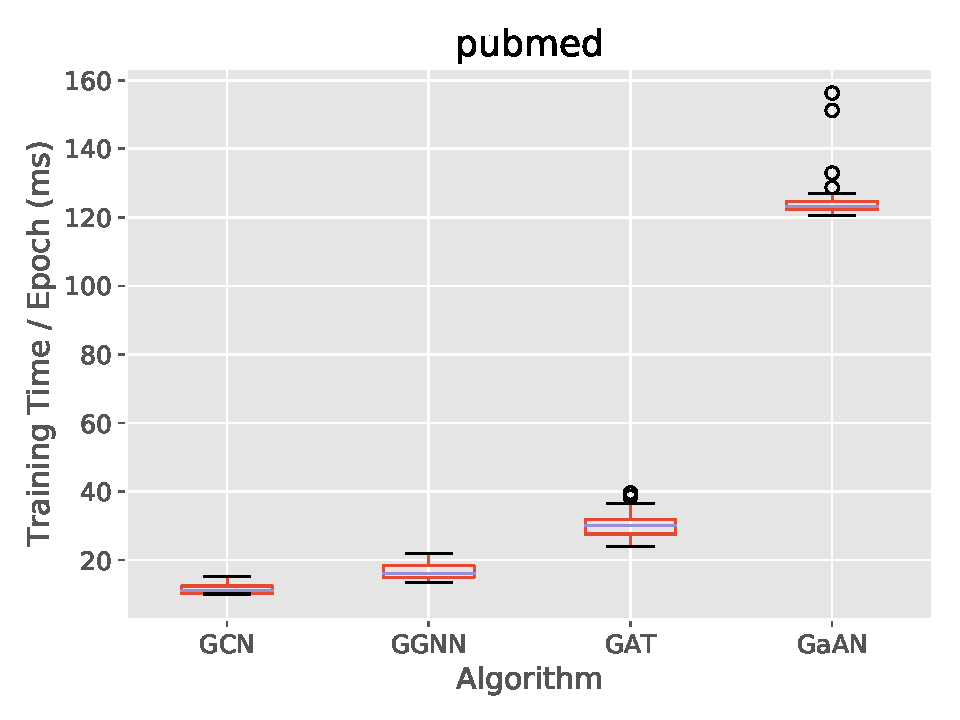
\includegraphics[height=4cm]{figs/experiments/exp_absolute_training_time_comparison_pubmed.pdf}}
    \subfloat[\texttt{aph}\label{fig:exp_absolute_training_time_amazon-photo}]{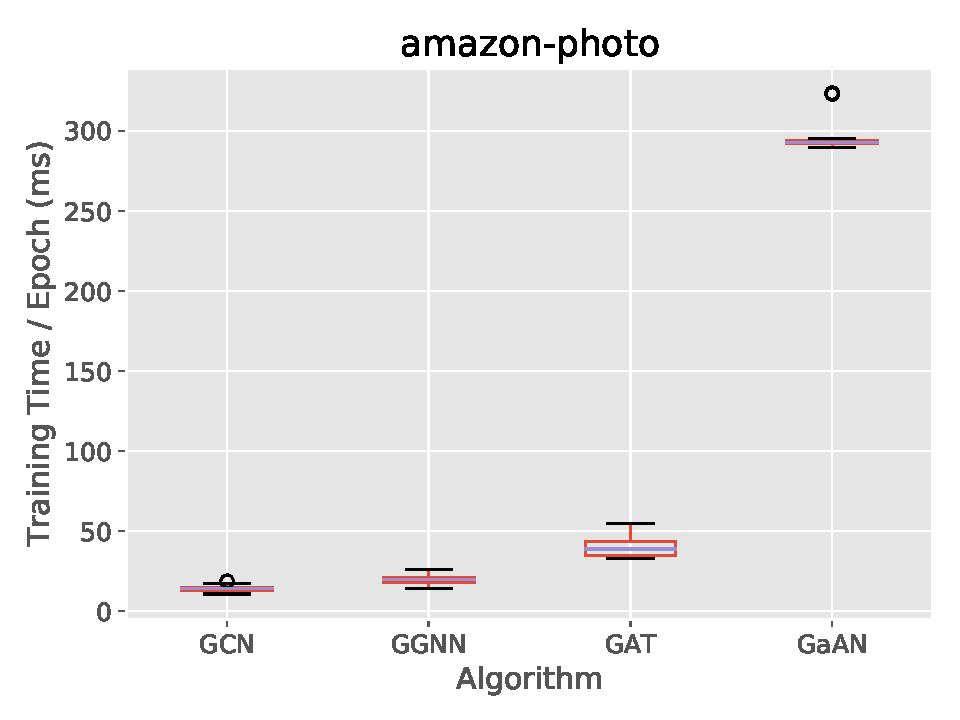
\includegraphics[height=4cm]{figs/experiments/exp_absolute_training_time_comparison_amazon-photo.pdf}}
    \subfloat[\texttt{cph}\label{fig:exp_absolute_training_time_coauthor-physics}]{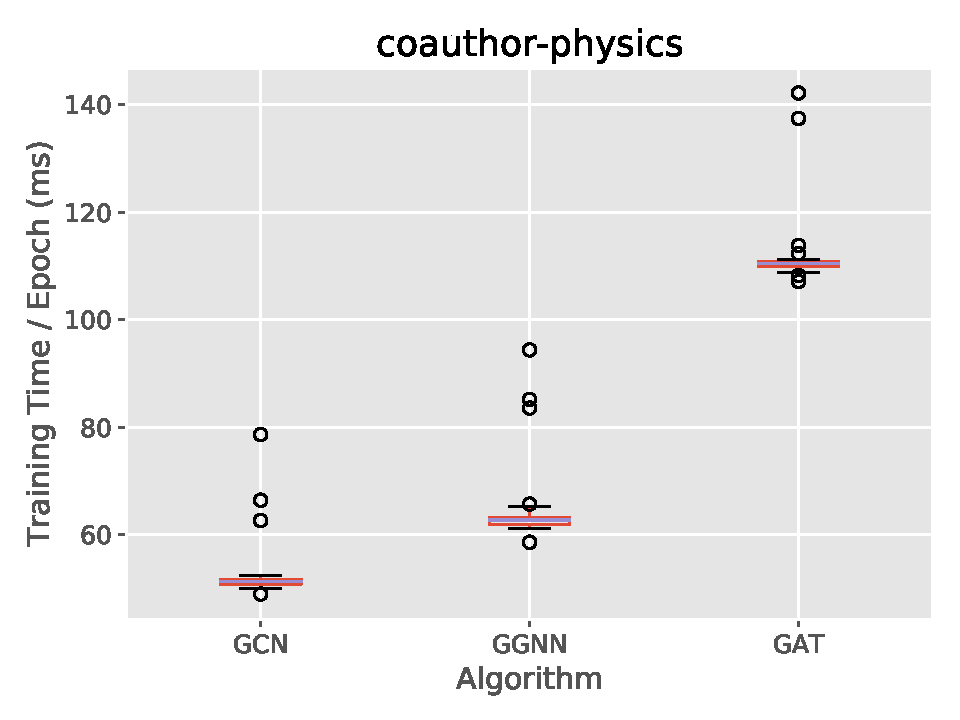
\includegraphics[height=4cm]{figs/experiments/exp_absolute_training_time_comparison_coauthor-physics.pdf}} \\
    \subfloat[\texttt{amc}\label{fig:exp_absolute_training_time_amazon-computers}]{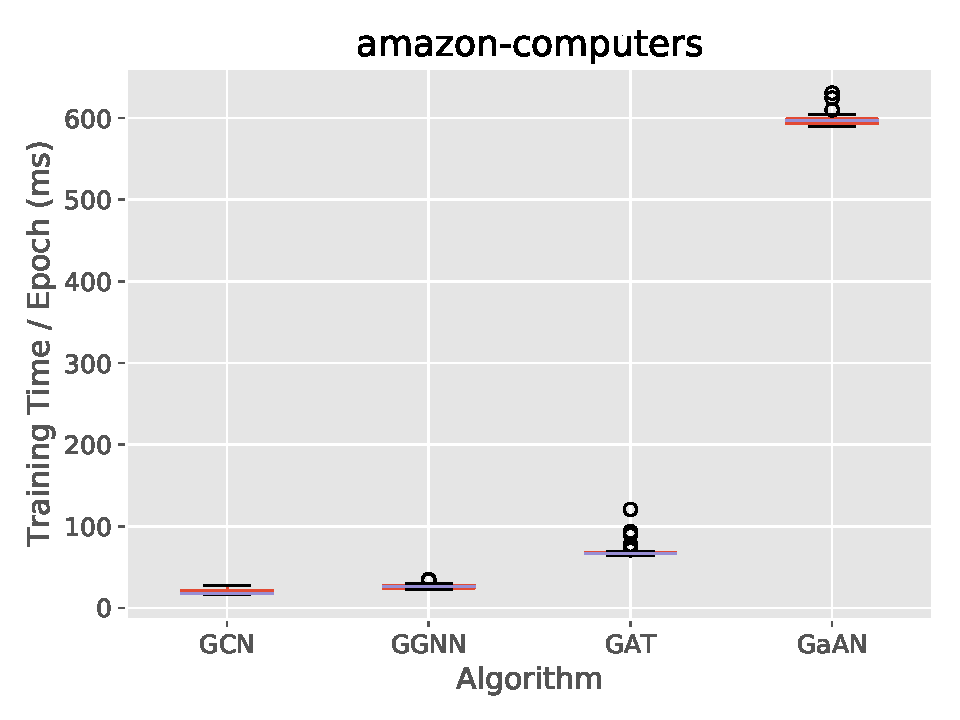
\includegraphics[height=4cm]{figs/experiments/exp_absolute_training_time_comparison_amazon-computers.pdf}}
    \subfloat[\texttt{fli}\label{fig:exp_absolute_training_time_flickr}]{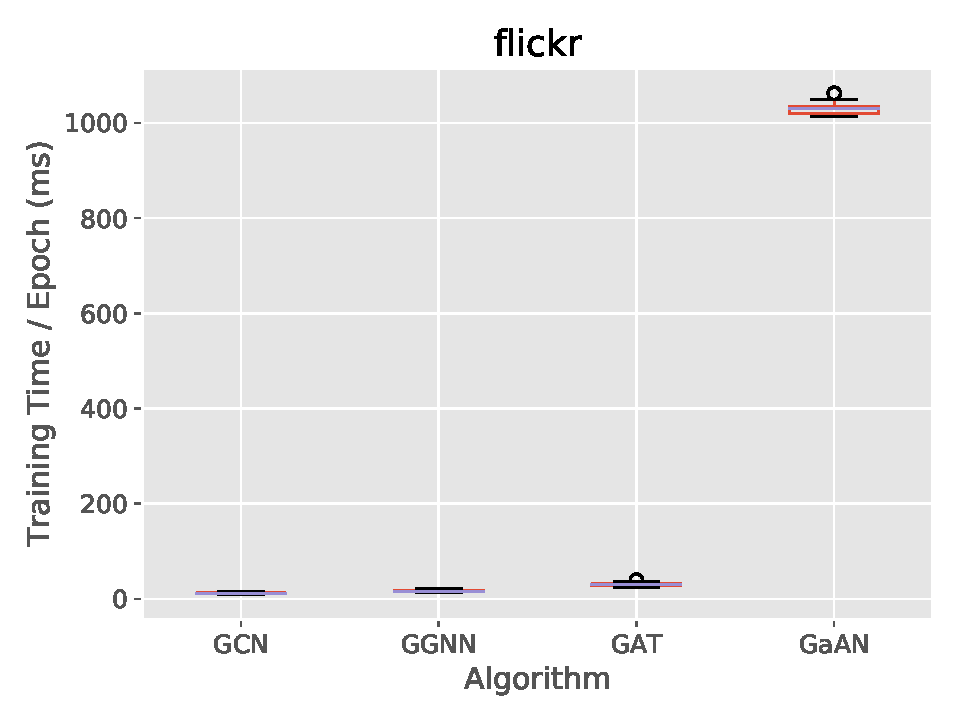
\includegraphics[height=4cm]{figs/experiments/exp_absolute_training_time_comparison_flickr.pdf}}
    \subfloat[\texttt{cam}\label{fig:exp_absolute_training_time_com-amazon}]{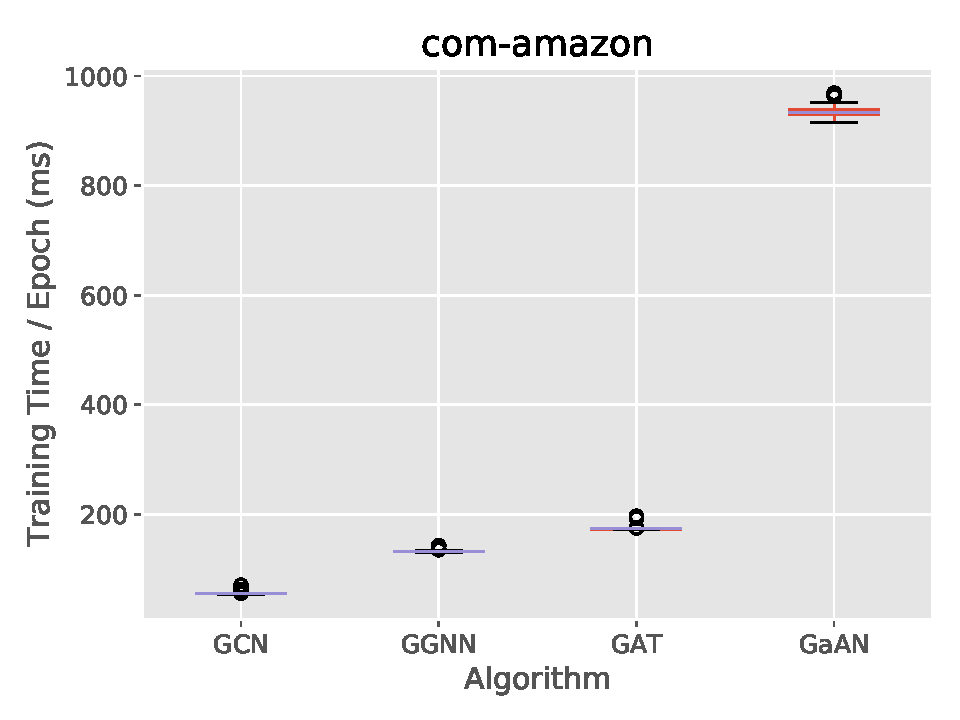
\includegraphics[height=4cm]{figs/experiments/exp_absolute_training_time_comparison_com-amazon.pdf}}
    \caption{Distribution of the wall-clock training time of 50 epoches on different datasets. GaAN crashed due to out of memory exception on the \texttt{cph} dataset.}
    \label{fig:exp_absolute_training_time}
\end{figure}

To further evaluate the effects of the hyper-parameters, we measure the training time of each GNN with varying hyper-parameters in \figurename~\ref{fig:exp_hyperparameter_on_vertex_edge_phase_time}.

\begin{figure}[tbp]
    \centering
    \subfloat[GCN\label{fig:exp_hyperparameter_on_vertex_edge_phase_time_gcn}]{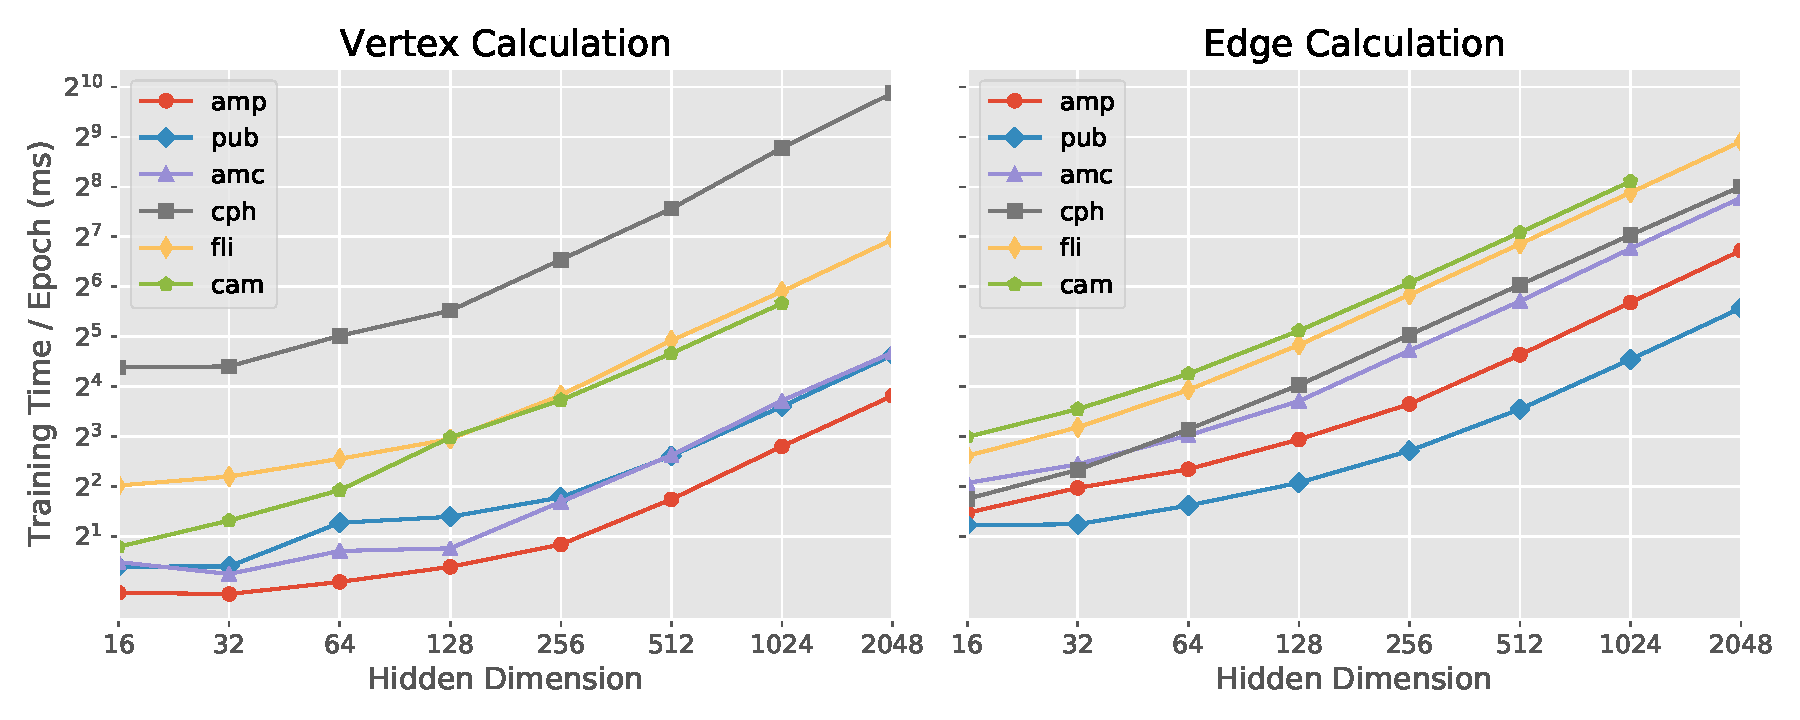
\includegraphics[height=3cm]{figs/experiments/exp_hyperparameter_on_vertex_edge_phase_time_gcn.pdf}}
    %
    \subfloat[GGNN\label{fig:exp_hyperparameter_on_vertex_edge_phase_time_ggnn}]{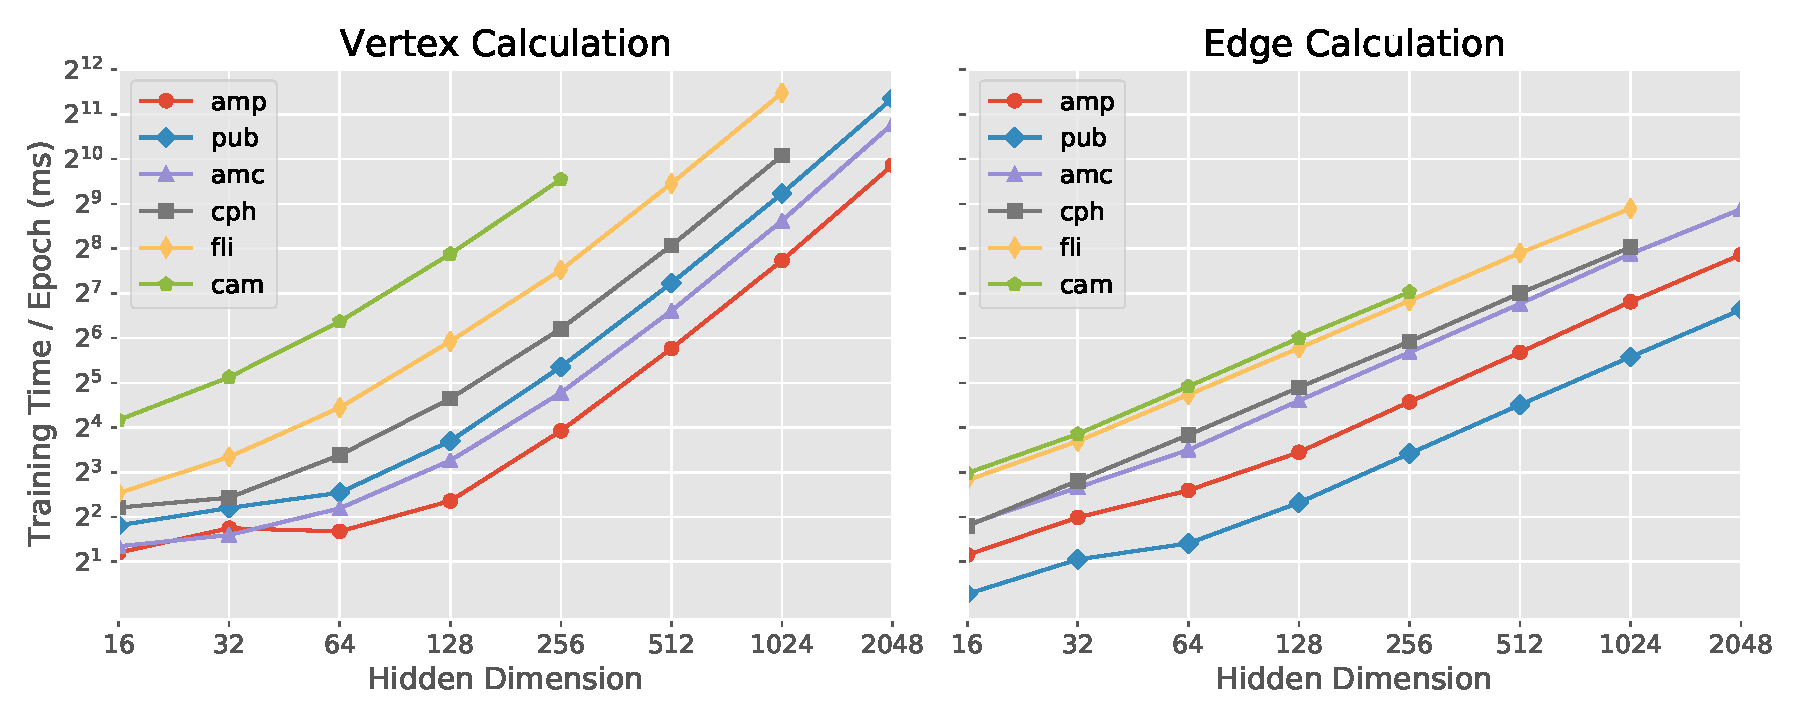
\includegraphics[height=3cm]{figs/experiments/exp_hyperparameter_on_vertex_edge_phase_time_ggnn.pdf}}
    \\
    \subfloat[GAT\label{fig:exp_hyperparameter_on_vertex_edge_phase_time_gat}]{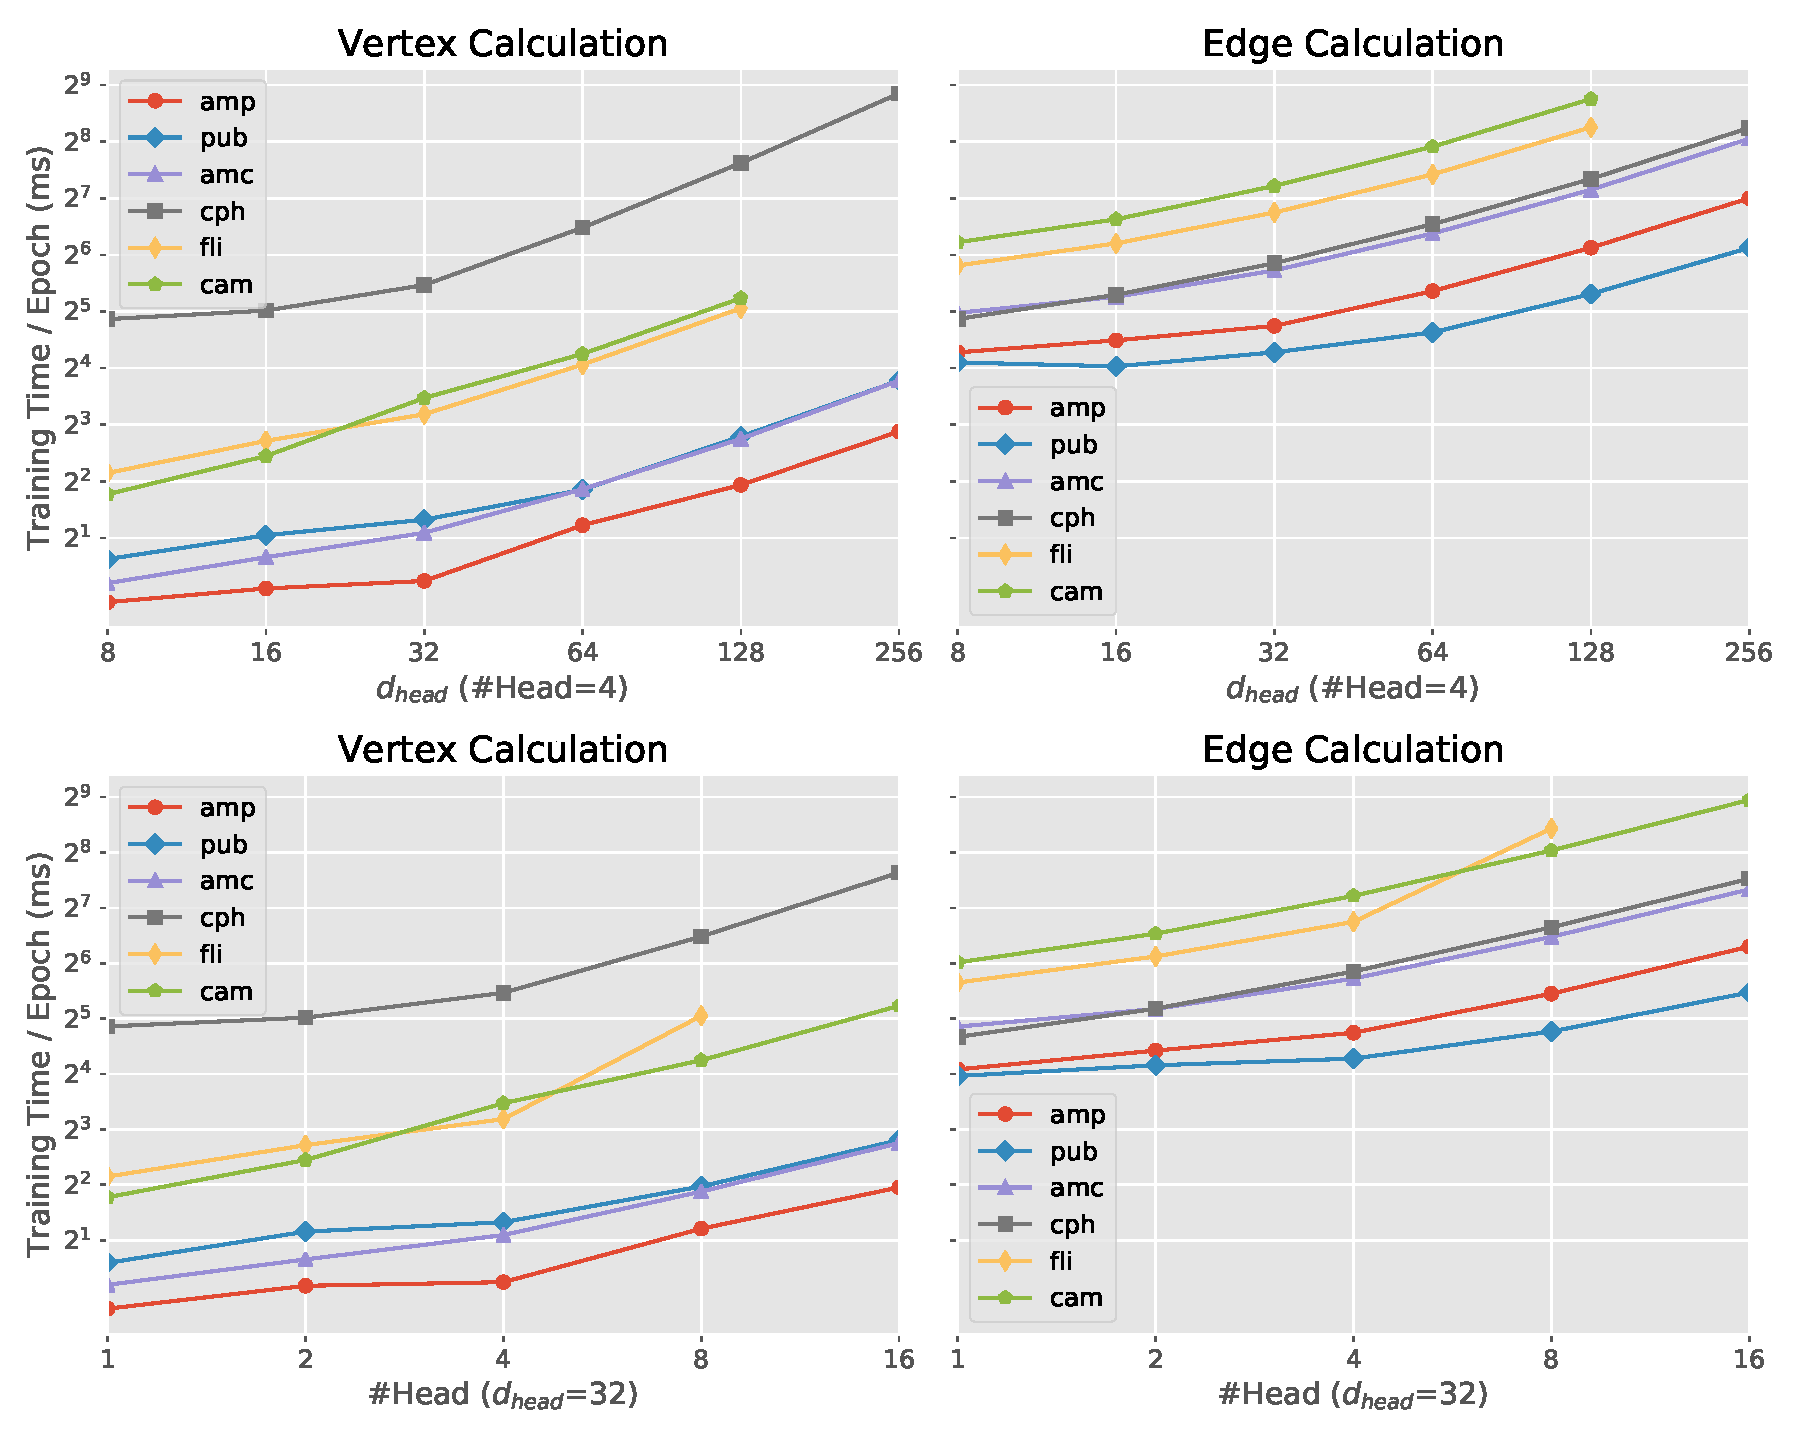
\includegraphics[height=6cm]{figs/experiments/exp_hyperparameter_on_vertex_edge_phase_time_gat.pdf}}
    \\
    \subfloat[GaAN\label{fig:exp_hyperparameter_on_vertex_edge_phase_time_gaan}]{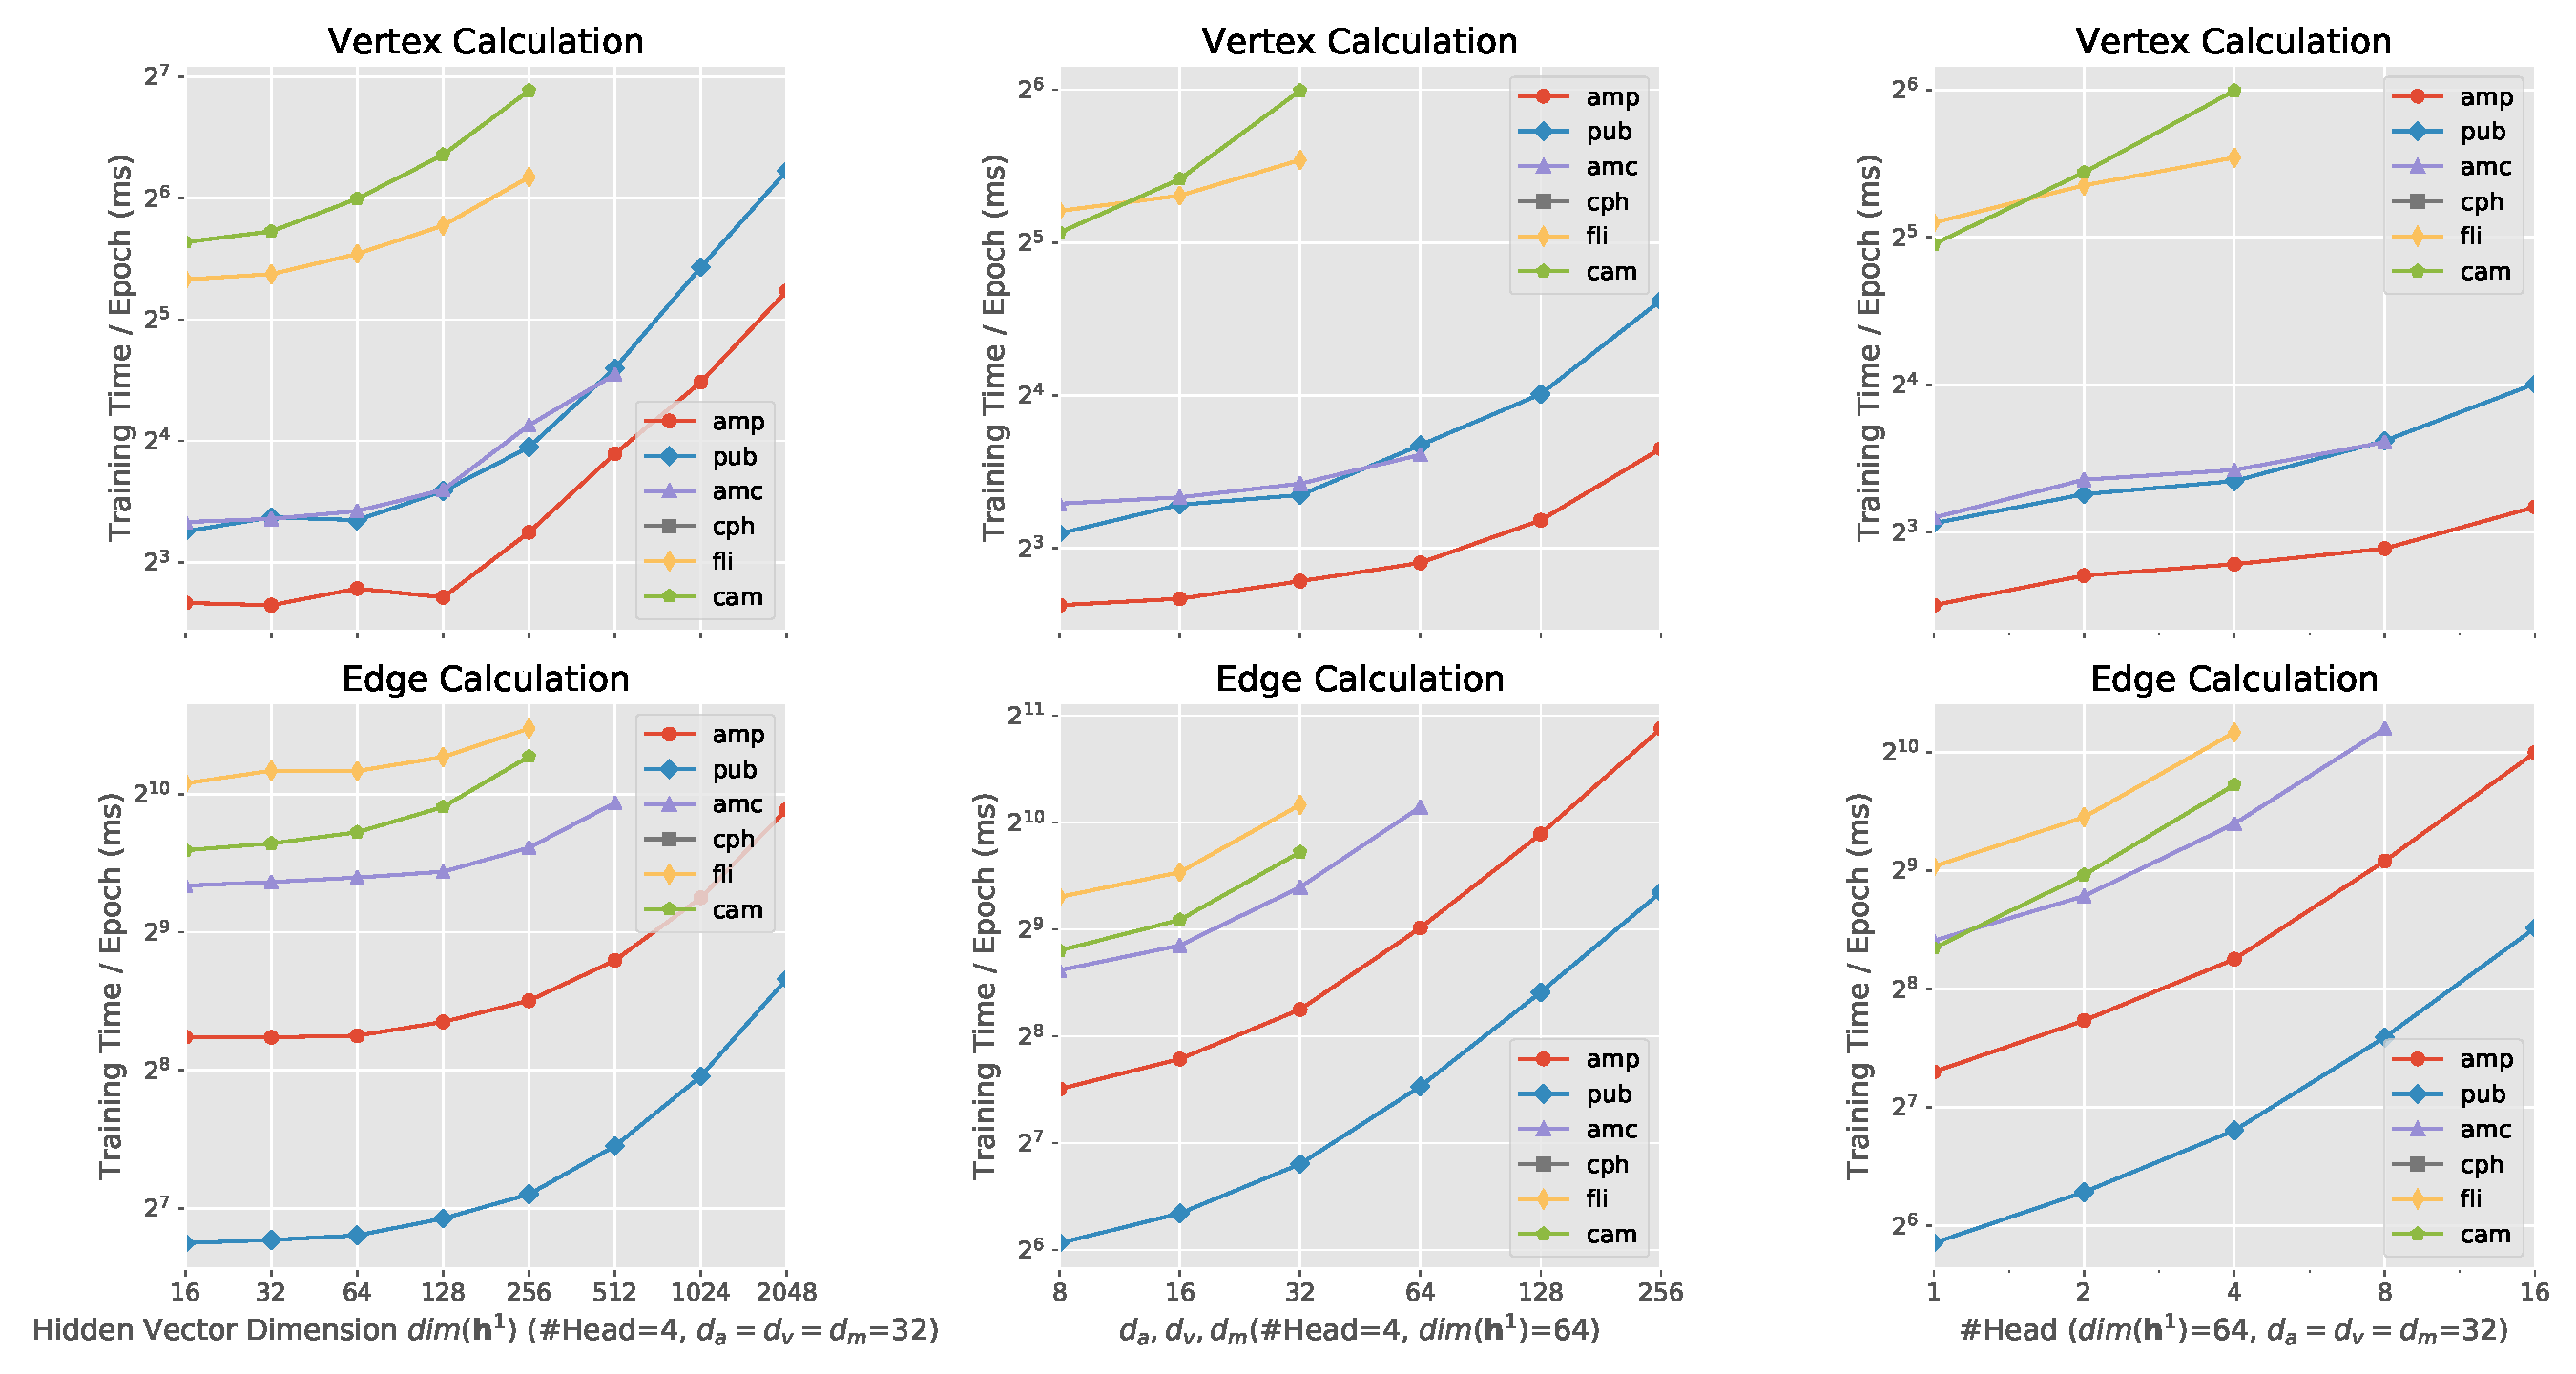
\includegraphics[height=6cm]{figs/experiments/exp_hyperparameter_on_vertex_edge_phase_time_gaan.pdf}}

    \caption{Effects of hyper-parameters on the edge/vertex calculation time.}
    \label{fig:exp_hyperparameter_on_vertex_edge_phase_time}
\end{figure}


Since $dim(\boldsymbol{h^0})$ and $dim{\boldsymbol{h^1}}$ are determined by the dataset with $dim(\boldsymbol{h}^0=dim(\boldsymbol{x}))$ and $dim(\boldsymbol{h}^2)=\#Classes$,
for GCN and GGNN, the only modifiable hyper-parameter is the hidden dimension $dim(\boldsymbol{h}^1)$ with $dim(\boldsymbol{h}^1) = d^0_{out} = d^1_{in}$.
According to the time complexity analysis, if we fix other hyper-parameters but only increase $dim(\boldsymbol{h}^1)$, the computing costs of the GNN layer 0 and the GNN layer 1 both increase linearly with $dim(\boldsymbol{h}^1)$, causing the training time of the whole GNN also increasing linearly. 
\figurename~\ref{fig:exp_hyperparameter_on_vertex_edge_phase_time_gcn} and \figurename~\ref{fig:exp_hyperparameter_on_vertex_edge_phase_time_ggnn} show that the training time of GCN and GGNN increased linearly with $dim(\boldsymbol{h}^1)$ when $dim(\boldsymbol{h}^1)$ is big, consistent with the time complexity analysis.

For GAT, we modify the number of heads $K$ and the dimension of each head $d_{head}$ in the GAT layer 0.
The dimension of the hidden feature vector is determined correspondingly as $d^0_{out} = d^1_{in} = dim(\boldsymbol{h}^1) = K d_{head}$.
Thus, the computing costs of the GAT layer 0 and the GAT layer 1 increase linearly with K and $d_{head}$ separately. 
\figurename~\ref{fig:exp_hyperparameter_on_vertex_edge_phase_time_gat} confirms the theoretical analysis.

For GaAN, it is also based on the multi-head mechanism.
Its time complexity is affected by $dim(\boldsymbol{h}^1)$ ($d^0_{out} = d^1_{in} = dim(\boldsymbol{h}^1)$), $d_a$, $d_v$, $d_m$ and the number of heads $K$.
\figurename~\ref{fig:exp_hyperparameter_on_vertex_edge_phase_time_gaan} demonstrates that the training time increases linearly with the hyper-parameters, except for $dim(\boldsymbol{h}^1)$.
As $dim(\boldsymbol{h}^1)$ increases, the training time increases first slightly and then linearly.
We observe similar phenomena in GCN, GGNN, and GAT with low hyper-parameters.
When the hyper-parameters is too low, the GNN training cannot make full use of the computing power of the GPU.
When the hyper-parameter becomes high enough, the training time increases linearly, supporting the time complexity analysis.

\begin{figure}[tbp]
    \centering
    \subfloat[GCN]{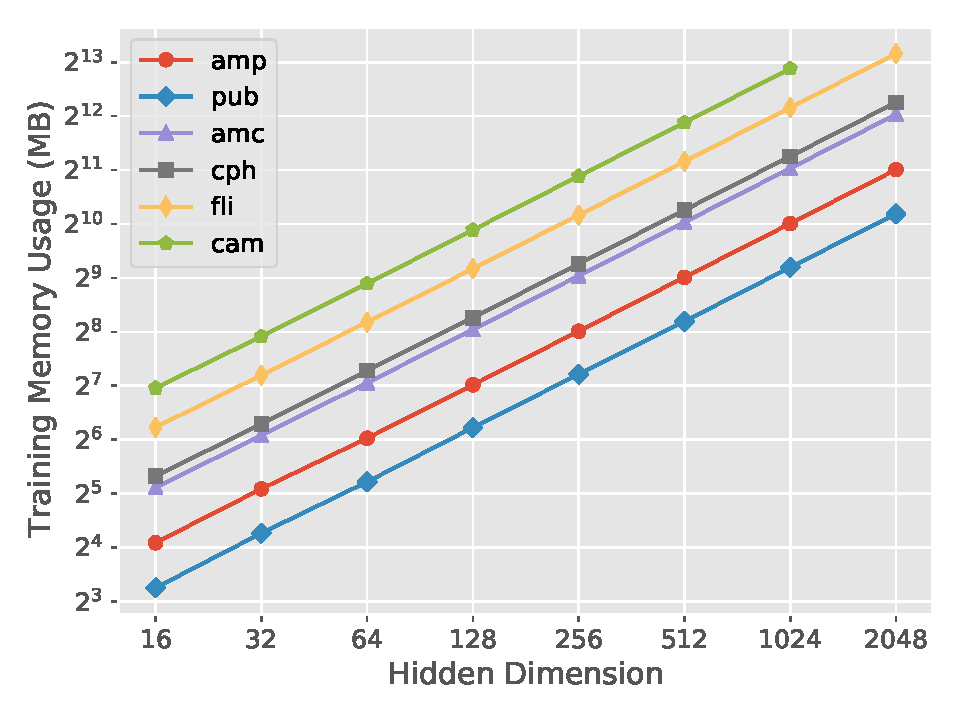
\includegraphics[height=3cm]{figs/experiments/exp_hyperparameter_on_memory_usage_gcn.pdf}}
    \subfloat[GGNN]{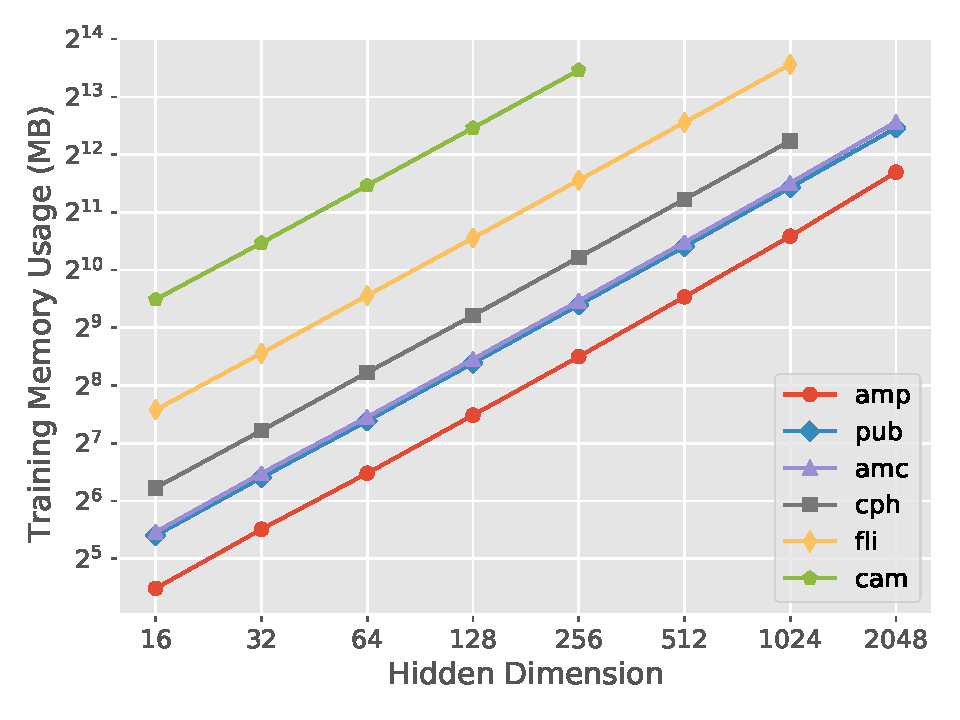
\includegraphics[height=3cm]{figs/experiments/exp_hyperparameter_on_memory_usage_ggnn.pdf}}\\
    \subfloat[GAT]{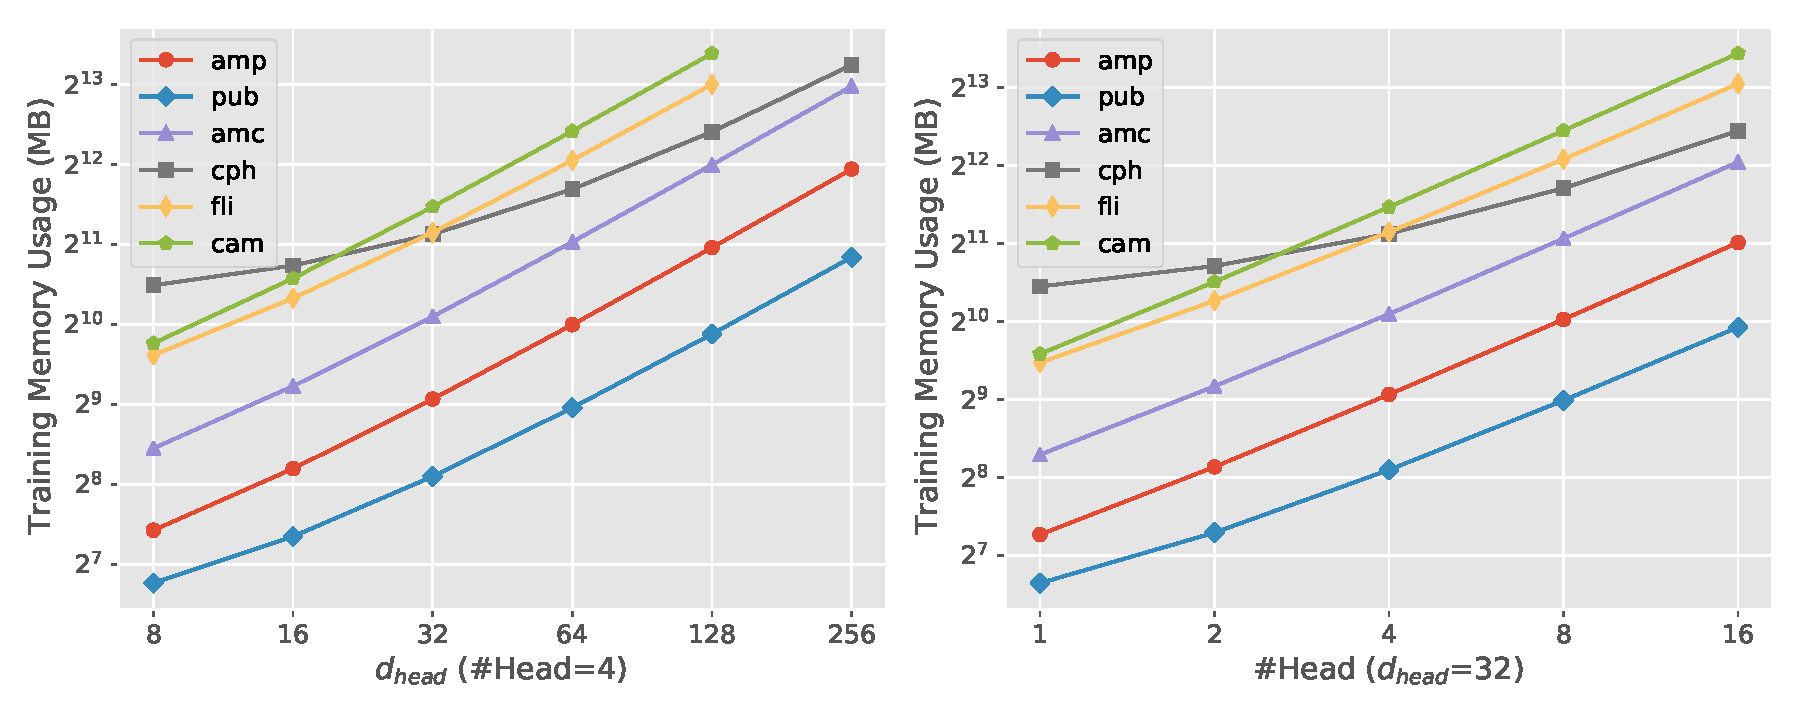
\includegraphics[height=3cm]{figs/experiments/exp_hyperparameter_on_memory_usage_gat.pdf}}\\
    \subfloat[GaAN]{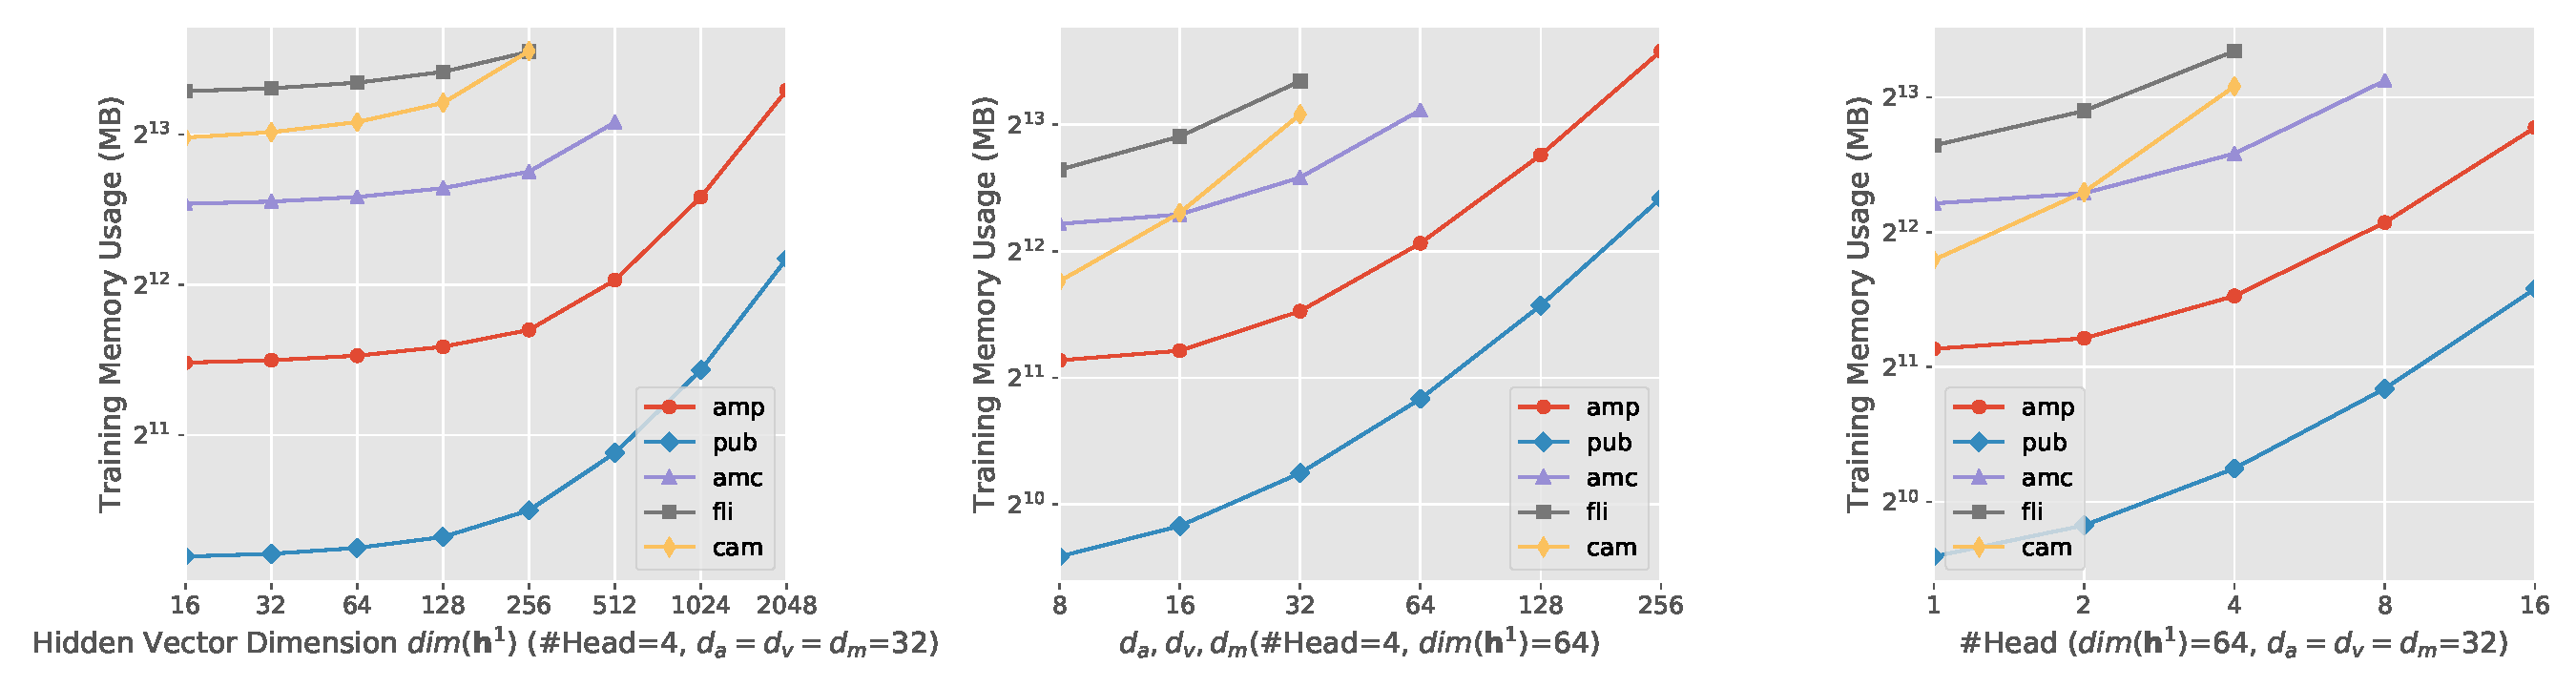
\includegraphics[height=3cm]{figs/experiments/exp_hyperparameter_on_memory_usage_gaan.pdf}}
    \caption{Effects of hyper-parameters on the peak GPU memory usage during the training, excluding the memory used by the dataset and the model parameters.}
    \label{fig:exp_hyperparameter_memory_usage}
\end{figure}

We further measured the effects of the hyper-parameters on the peak GPU memory usage in \figurename~\ref{fig:exp_hyperparameter_memory_usage}.
The memory usage also increases linearly as the hyper-parameters increase for all GNNs, except for GaAN on $dim(\boldsymbol{h}^1)$.
As the hidden feature vectors $\boldsymbol{h}^1$ consume a small proportion of memory in GaAN, the growth in the memory usage is not noticeable until $dim(\boldsymbol{h}^1)$ is large enough.

\paragraph{Summary}

The complexity analysis in \tablename~\ref{tab:gnn_overview_edge} and \tablename~\ref{tab:gnn_overview_vertex} is valid.
Fixing other hyper-parameters, each hyper-parameter, itself affects the training time and the memory usage of a GNN Layer \textbf{in a linear way}.
Algorithm engineers can adjust hyper-parameters according to the time complexity to avoid explosive growth in the training time and memory usage.

\subsection{Training Time Breakdown}
\label{sec:training_time_breakdown}

To find out which stage/step dominates the training time, we decompose the training time and analyze the performance bottleneck level by level.

\subsubsection{Layer Level}

\begin{figure}[tbp]
    \centering
    \subfloat[GCN]{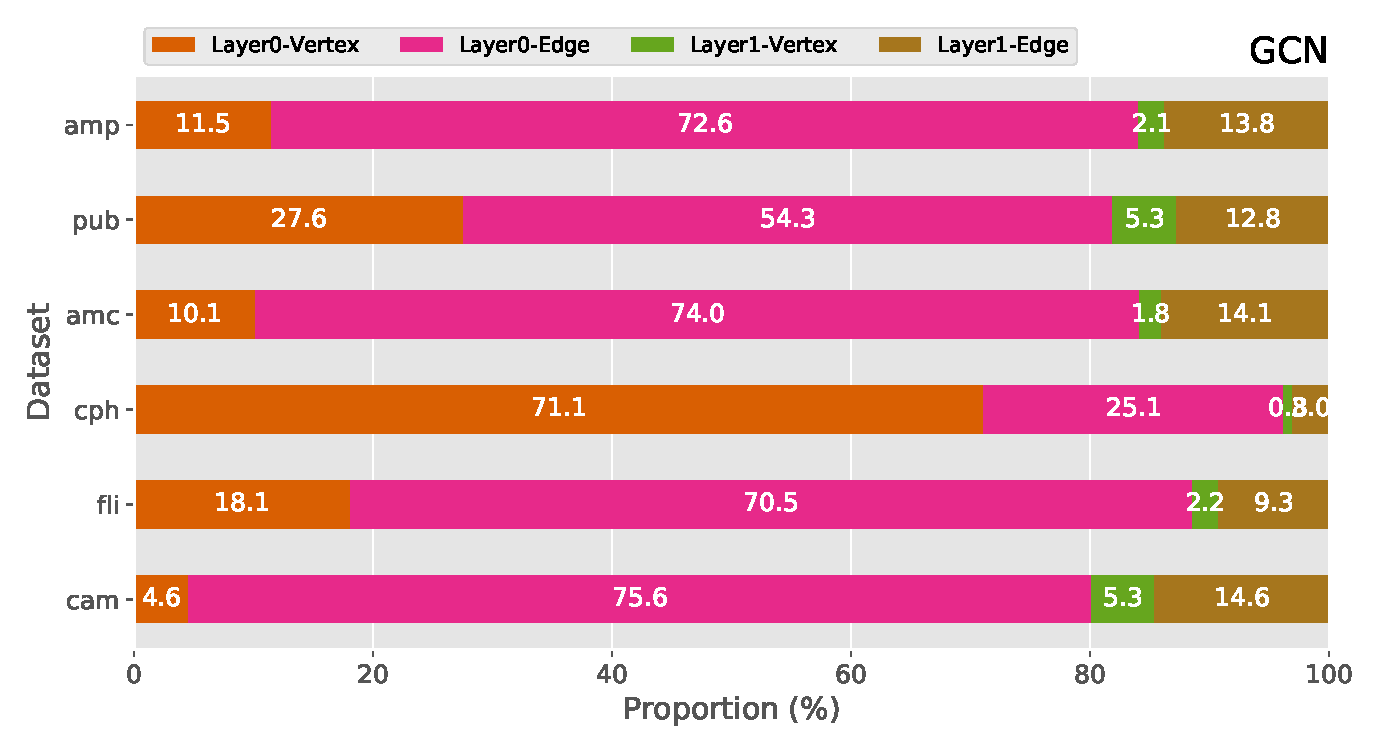
\includegraphics[height=4cm]{figs/experiments/exp_layer_time_proportion_gcn.pdf}}
    \subfloat[GGNN]{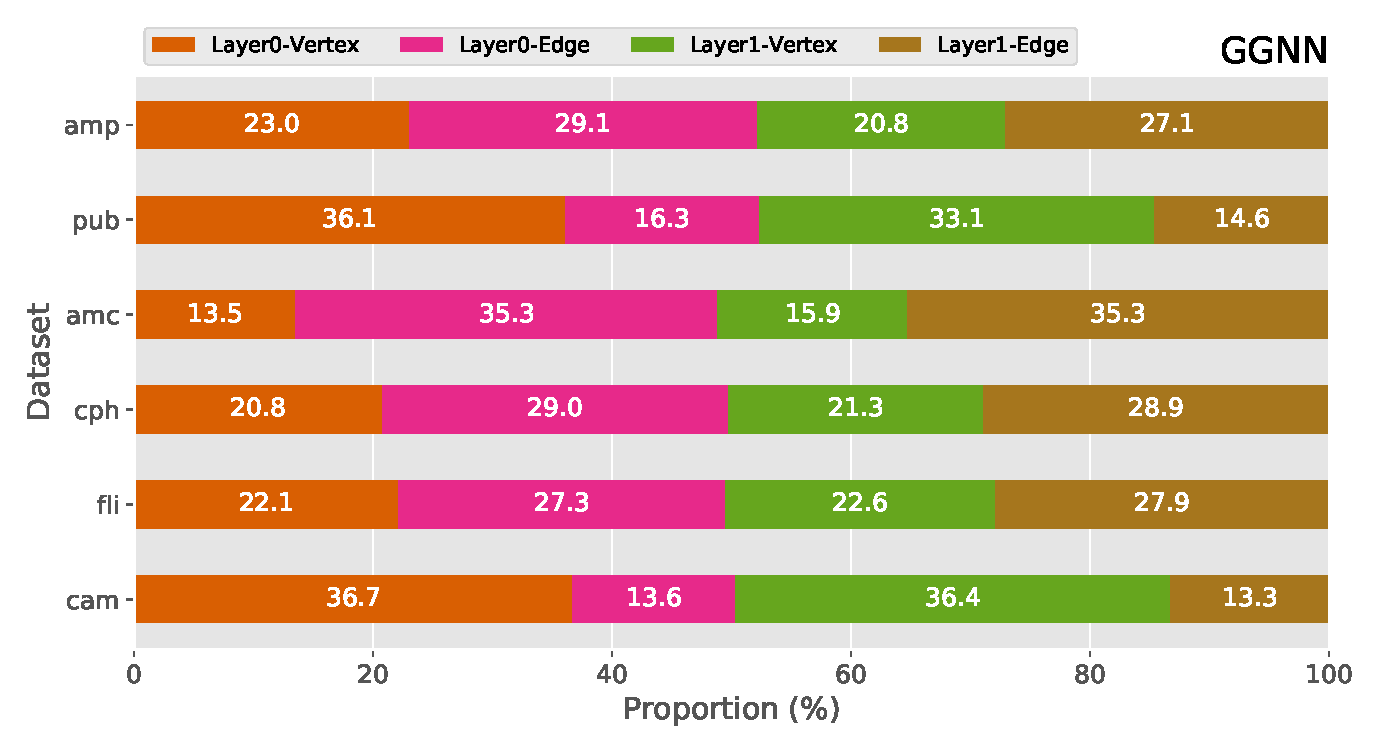
\includegraphics[height=4cm]{figs/experiments/exp_layer_time_proportion_ggnn.pdf}}\\
    \subfloat[GAT]{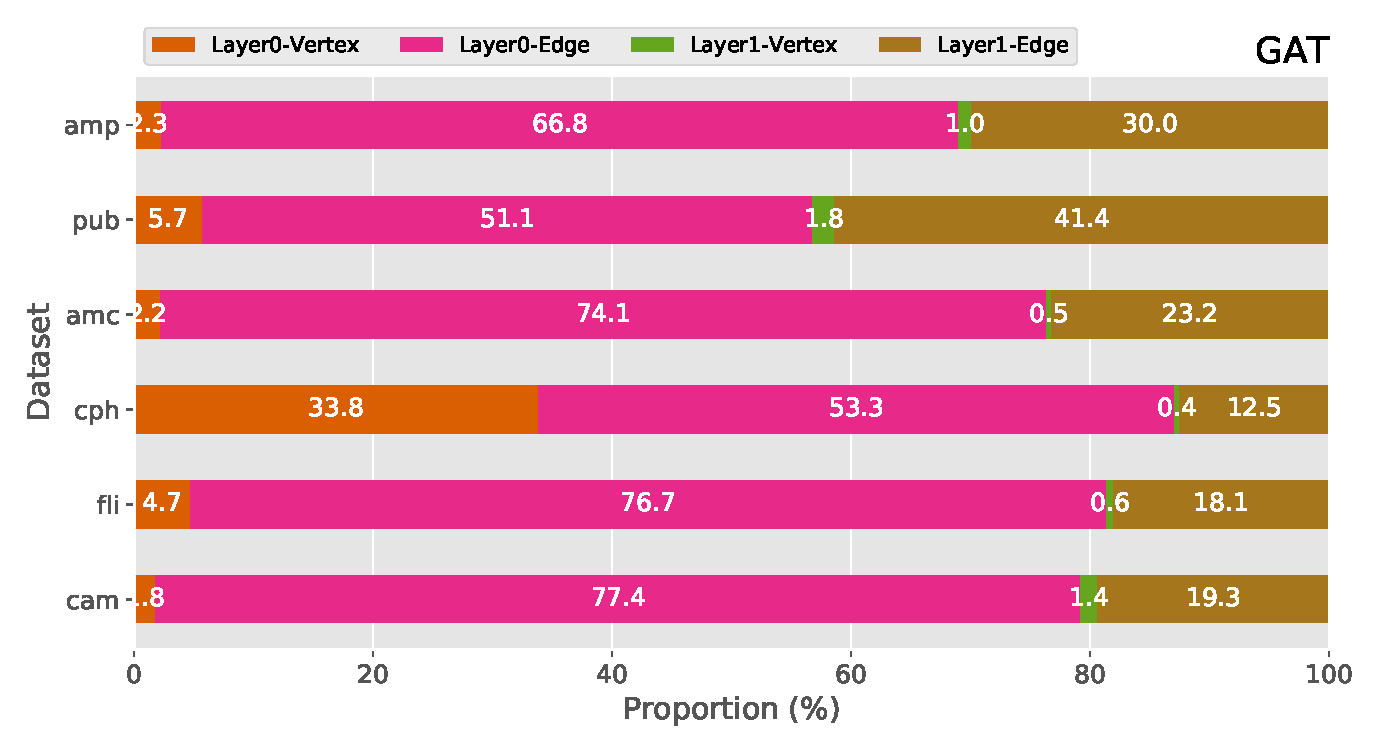
\includegraphics[height=4cm]{figs/experiments/exp_layer_time_proportion_gat.pdf}}
    \subfloat[GaAN]{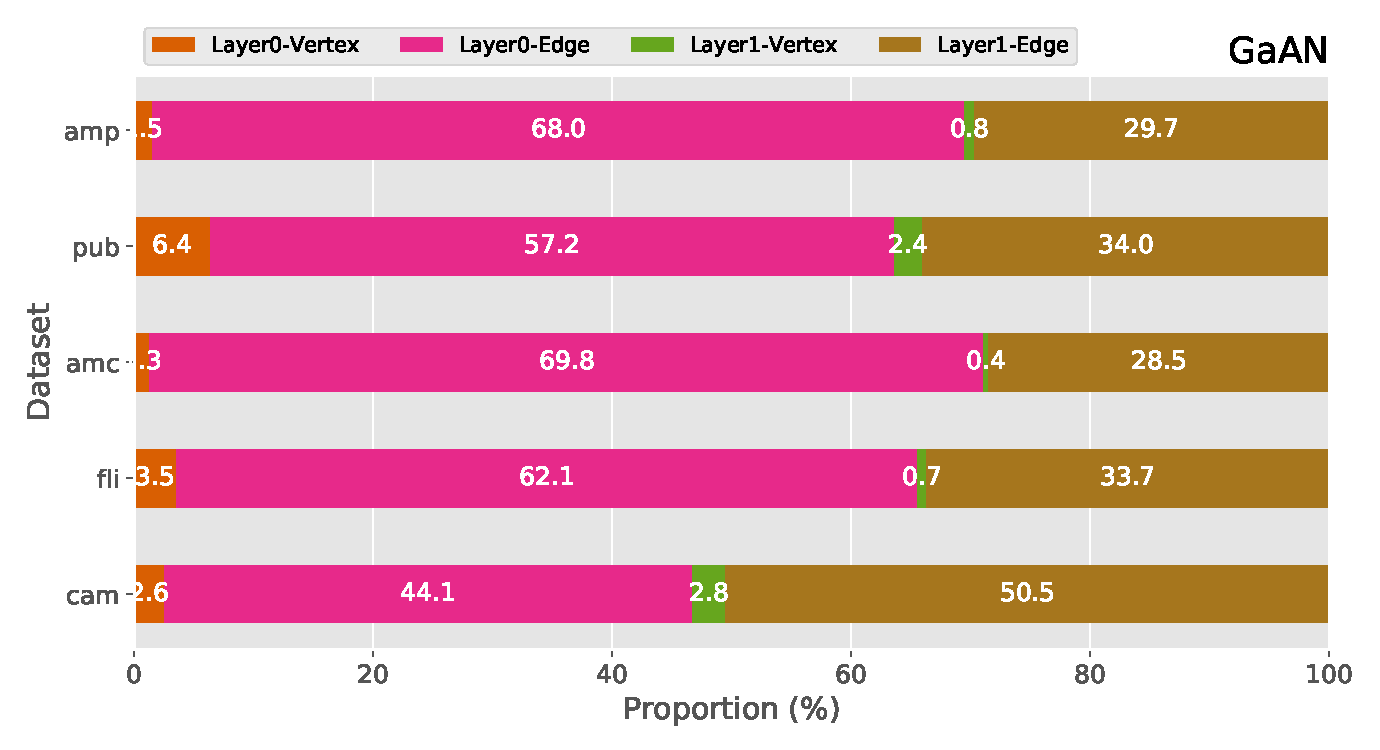
\includegraphics[height=4cm]{figs/experiments/exp_layer_time_proportion_gaan.pdf}}
    \caption{Training time breakdown on the layer level. The training time of each layer includes the time spent on the forward, backward and evaluation phases. Each layer is further decomposed into the vertex and the edge calculation stages.}
    \label{fig:exp_vertex_edge_cal_proportion}
\end{figure}

\figurename~\ref{fig:exp_vertex_edge_cal_proportion} decomposes the training time of a GNN on the layer level.
The training time of each layer is the summation of the time in the forward, backward, and evaluation phases.
In GCN, GAT, and GaAN, the time spent on the layer 0 is much larger than the layer 1.
In those GNNs, the dimensions of the input/output feature vectors in the layer 0 are much larger than the dimensions in the layer 1.
$d^0_{in}=dim(\boldsymbol{x})$, $d^0_{out}=d^1_{in}=64$ and $d^1_{out}=\#Class$ and $dim(\boldsymbol{x}) \gg \#Class$.
For GaAN, since it requires the dimensions of the input/output feature vectors must be the same, the hyper-parameter are $d^0_{in}=d^0_{out}=d^1_{in}=d^1_{out}=64$ and the training time of both layers is close.

Each GNN layer can be further divided into the vertex and the edge calculation stages.
In \figurename~\ref{fig:exp_vertex_edge_cal_proportion}, GCN spends most of the training time on the edge calculation stage in most datasets.
A special case is \texttt{cph} dataset.
The dimension of the input feature vectors is very high in \texttt{cph}, making the vertex calculation stage of the GCN Layer 0 spend considerable time.
GGNN also spends the majority of its training time on the edge calculation stage.
But the high time complexity of its vertex updating function $\gamma$ makes the ratio of the vertex calculation in the total training time much higher than the other GNNs.
%In \textit{pub} and cam dataset, the edge calculation cost, and the vertex calculation cost are close for GGNN
%because the average degree of the two datasets is low (only 4.5 and 2.8).
For GAT and GaAN, due to their high edge calculation complexity, the edge calculation stage is the absolutely dominant stage.
In summary, \emph{the edge calculation stage is the most time-consuming stage in the GNN training}.

\begin{figure}[tbp]
    \centering
    \subfloat[GCN]{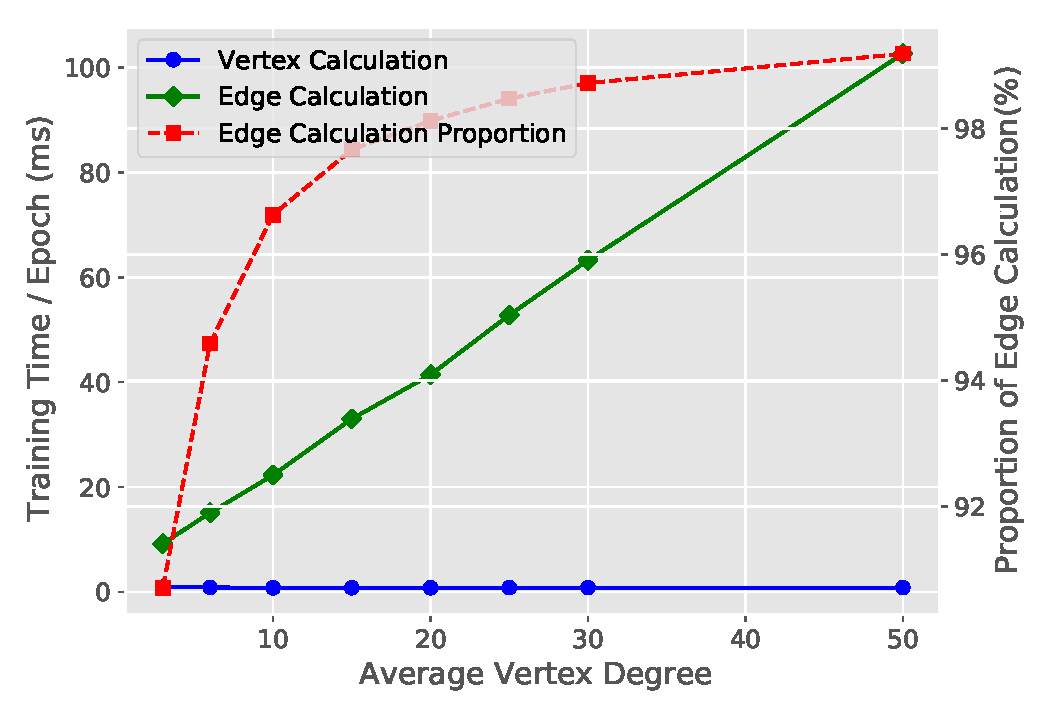
\includegraphics[height=4cm]{figs/experiments/exp_avg_degree_on_vertex_edge_cal_time_gcn.pdf}}
    \subfloat[GGNN]{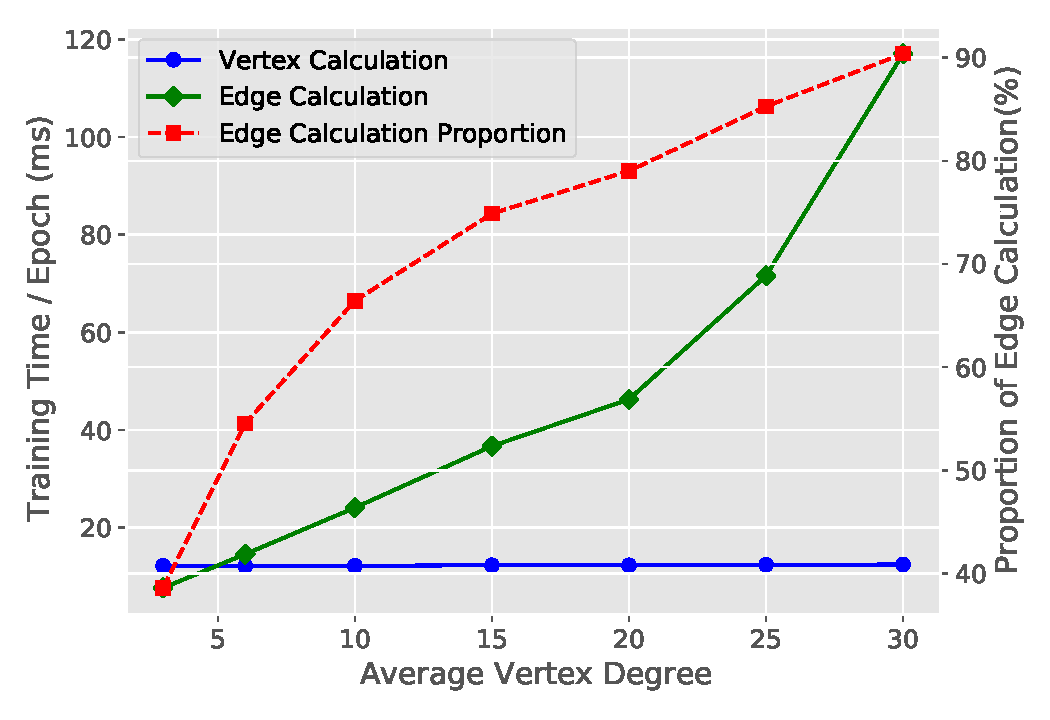
\includegraphics[height=4cm]{figs/experiments/exp_avg_degree_on_vertex_edge_cal_time_ggnn.pdf}}\\
    \subfloat[GAT]{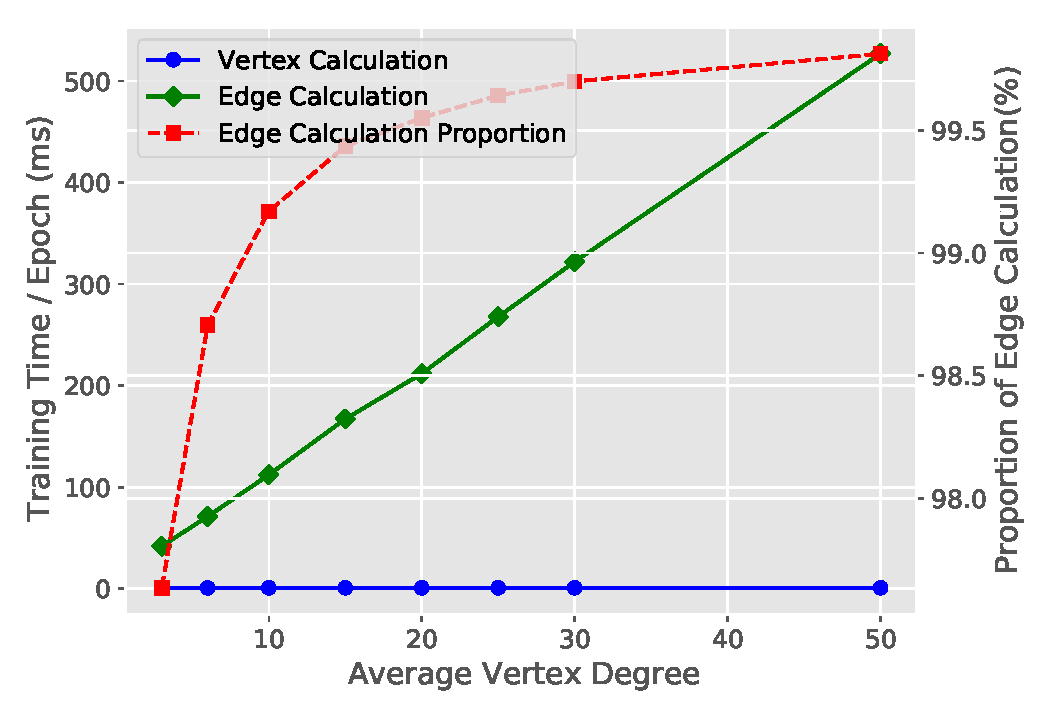
\includegraphics[height=4cm]{figs/experiments/exp_avg_degree_on_vertex_edge_cal_time_gat.pdf}}
    \subfloat[GaAN]{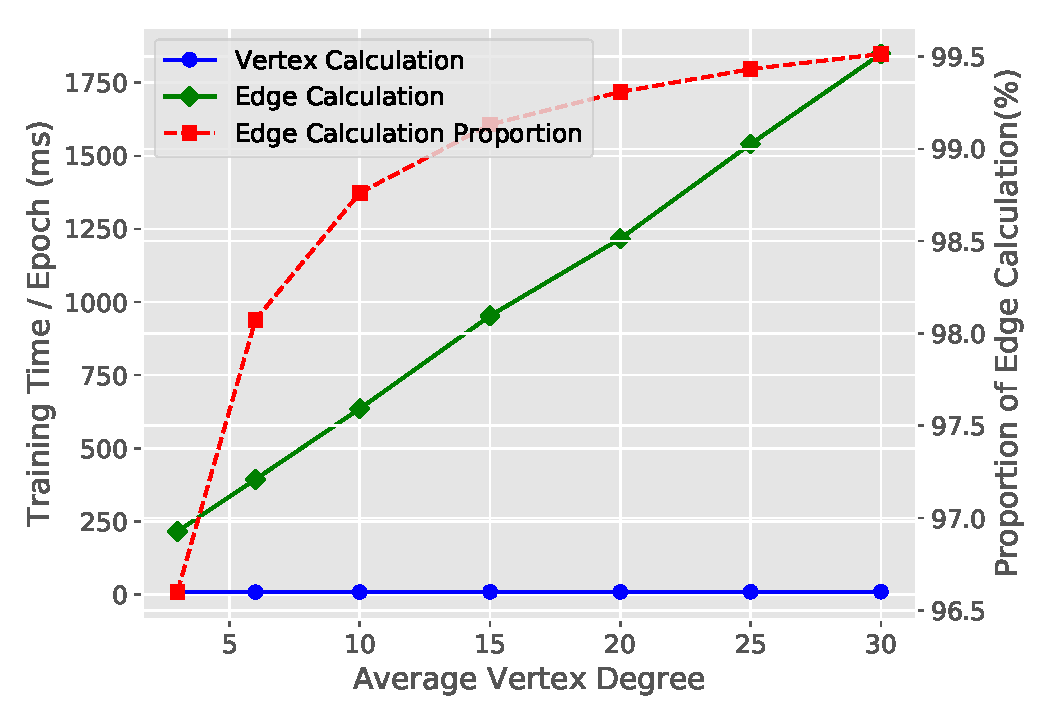
\includegraphics[height=4cm]{figs/experiments/exp_avg_degree_on_vertex_edge_cal_time_gaan.pdf}}
    \caption{Effects of the average degree on the time proportion of the edge/vertex calculation. Graphs were generated with the R-MAT generator by fixing the number of vertices as 50,000. }
    \label{fig:exp_avg_degree_on_vertex_edge_cal_time}
\end{figure}

The experimental results also indicate that the average degree of the dataset affects the time-consuming proportion of the edge/vertex calculation time.
For GaAN, the time spent on the vertex calculation stage exceeds the edge calculation stage on the \texttt{pub} and \texttt{cam} datasets, because the average degrees of the two datasets are low, making $|\mathcal{E}|$ and $|\mathcal{V}|$ much closer.
To evaluate the effects of the average degree, we used the R-MAT generator to generate random graphs with 50k vertices and the average degrees ranging from 2 to 100.
\figurename~\ref{fig:exp_avg_degree_on_vertex_edge_cal_time} shows the training time of the four GNNs under different average degrees.
As the average degree increases, the training time of the edge calculation stage grows \emph{linearly}.
For GCN, GAT, and GaAN, the edge calculation stage dominates the entire training time even under small average degrees.
Only for GGNN that has high vertex and low edge calculation complexities, the training time of the vertex calculation stage exceeds the edge calculation stage under low average degrees ($<5$).
Therefore, \emph{improving the efficiency of the edge calculation stage is the key to reduce the GNN training time}.

\subsubsection{Step Level in Edge Calculation}

\begin{figure}[tbp]
    \centering
    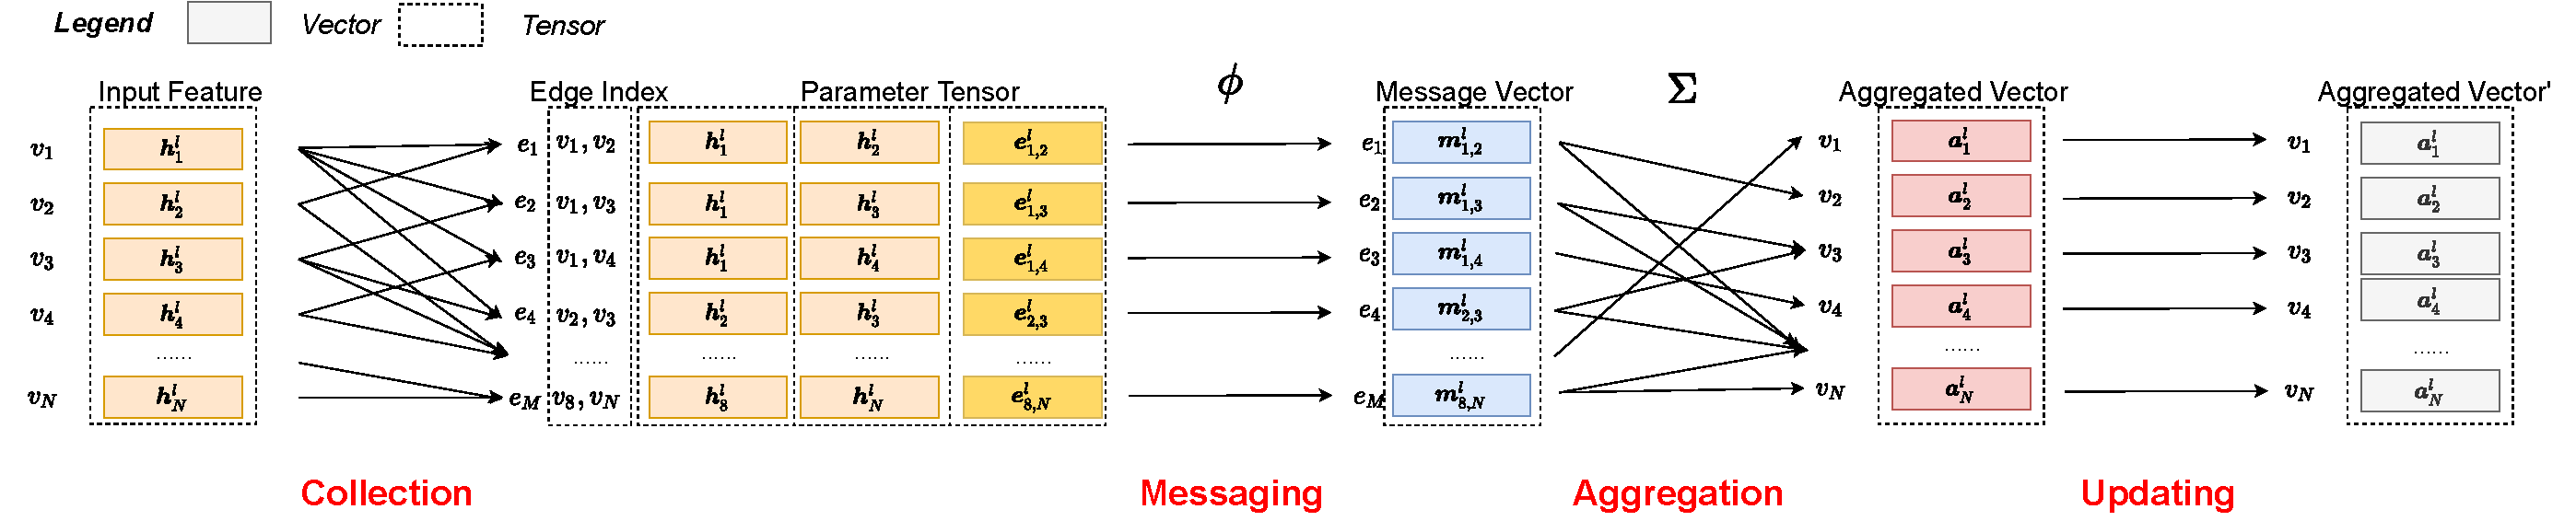
\includegraphics[width=1\columnwidth]{figs/illustration/steps_in_edge_calculation.pdf}
    \caption{Step decomposition of the edge calculation in the GNN layer $l$.}
    \label{fig:steps_in_edge_calculation}
\end{figure}

In the implementation of PyG, the edge calculation stage can be decomposed into four steps: collection, messaging, aggregation, and updating, as shown in \figurename~\ref{fig:steps_in_edge_calculation}.
The edge index is a matrix with $M$ rows and 2 columns that holds the edge set of the graph, where $M=|\mathcal{E}|$.
The two columns of the matrix store the source vertex and the target vertex of each edge, respectively.
The collection step copies the vertex feature vectors from the previous layer $\boldsymbol{h}_i^l$ to the ends of each edge
in the edge index, to form the parameters tensor $[\boldsymbol{h}^l_i, \boldsymbol{h}^l_{j}, \boldsymbol{e}^l_{i,j}]$ of the messaging function $\phi$.
This step only involves the data movement.
The messaging step calls the messaging function $\phi$ to get message vectors of all edges $\boldsymbol{m}_{i, j}^l$.
The aggregation step aggregates the message vectors with the same target vertex into an aggregated vector $\boldsymbol{s}^l_i$ with the aggregation operation $\Sigma$.
The updating step is optional.
It performs an additional transformation on the aggregated vectors (for example, adding bias in GCN).
The aggregated vectors $\boldsymbol{s}^l_i$ (after the updating step) will be fed into the vertex updating function $\gamma$ as one of the input parameters.

\begin{figure}[tbp]
    \centering
    \subfloat[GCN]{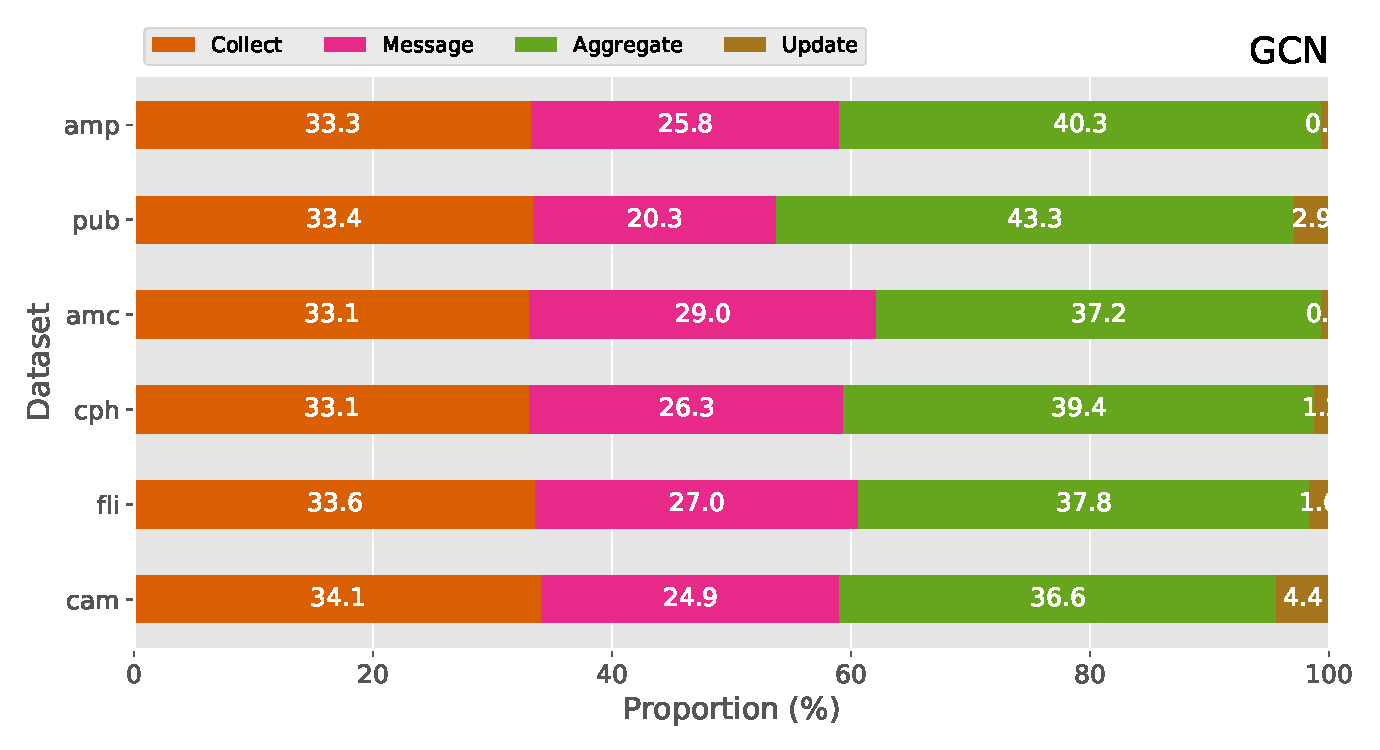
\includegraphics[height=4cm]{figs/experiments/exp_edge_calc_decomposition_gcn.pdf}}
    \subfloat[GGNN]{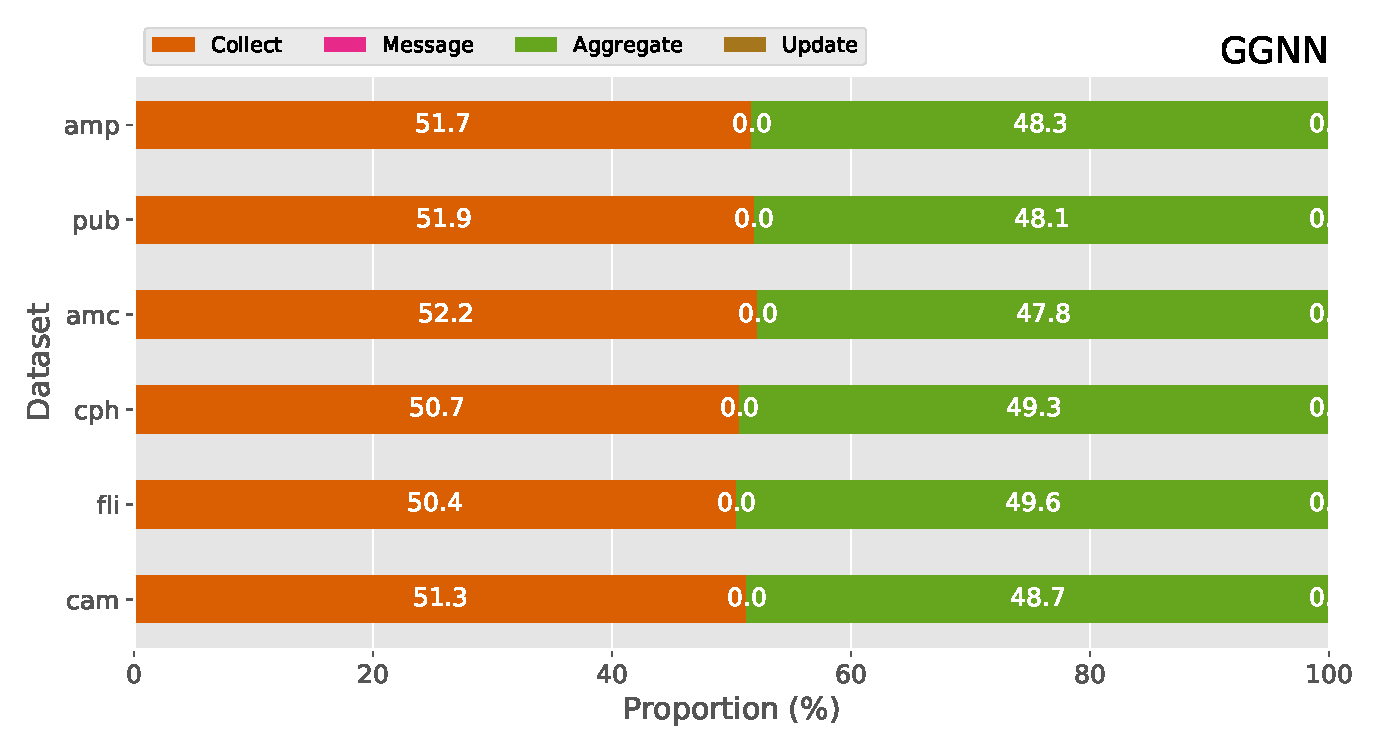
\includegraphics[height=4cm]{figs/experiments/exp_edge_calc_decomposition_ggnn.pdf}}\\
    \subfloat[GAT]{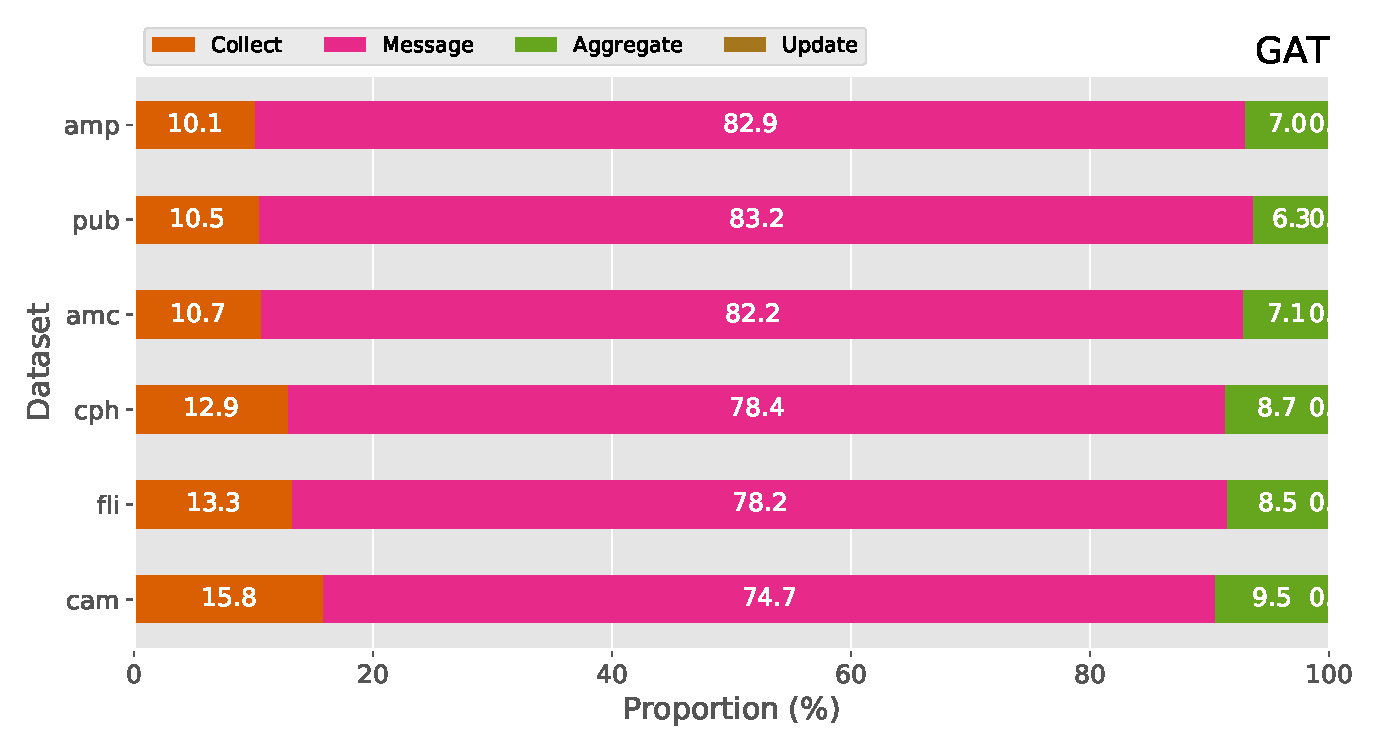
\includegraphics[height=4cm]{figs/experiments/exp_edge_calc_decomposition_gat.pdf}}
    \subfloat[GaAN]{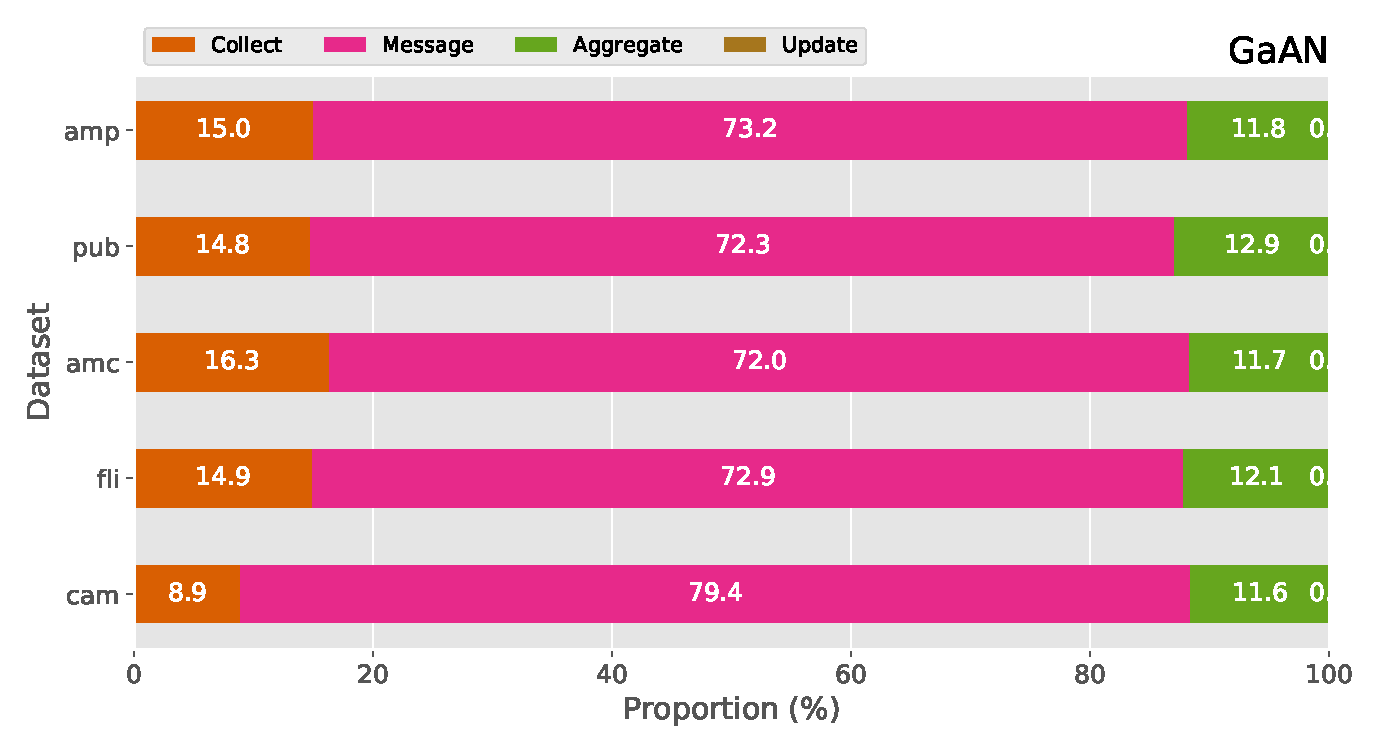
\includegraphics[height=4cm]{figs/experiments/exp_edge_calc_decomposition_gaan.pdf}}
    \caption{Training time breakdown of the edge calculation stage (including both GNN layers).}
    \label{fig:exp_edge_calc_decomposition}
\end{figure}

We decompose the execution time of the edge calculation stage in \figurename~\ref{fig:exp_edge_calc_decomposition}.
In each GNN, the proportions of the four steps are rather stable, rarely affected by datasets. 
For GAT and GaAN with the high edge calculation complexity, the messaging step consumes most of the training time. 
For GCN and GGNN with the low edge complexity, the proportions of the steps are close. 
Since the messaging function $\phi$ of GGNN uses the pre-computed $\hat{\boldsymbol{h}}^l_i$ as the message vector directly, the time spent on the messaging step of GGNN is negligible.
Although the collecting step does not conduct any computation and only involves data movement, it occupies noticeable execution time in all the GNNs.
The experiments show that \emph{the performance bottleneck on the step level depends on the complexity of the messaging function $\phi$}.
For GNNs with the high complexity, the messaging function $\phi$ is the performance bottleneck.
Optimizing the implementation of $\phi$ can significantly reduce the training time.
For the other GNNs, optimization should focus on reducing the costs of the collection and the aggregation steps.
Additionally, improving the efficiency of the collection step can benefit all GNNs.

\subsubsection{Operator Level}

The functions $\phi$, $\Sigma$ and $\gamma$ in the vertex and edge calculation are made up of a series of basic operators implemented on the GPU, like the matrix multiplication \texttt{mm}, the elementwise multiplication \texttt{mul} and the index-based selection \texttt{index\_select}.
\figurename~\ref{fig:exp_top_basic_ops} shows the five most time-consuming basic operators in each GNN, averaged over all the real-world graphs in \tablename~\ref{tab:dataset_overview}.

\begin{figure}[tbp]
    \centering
    \subfloat[GCN]{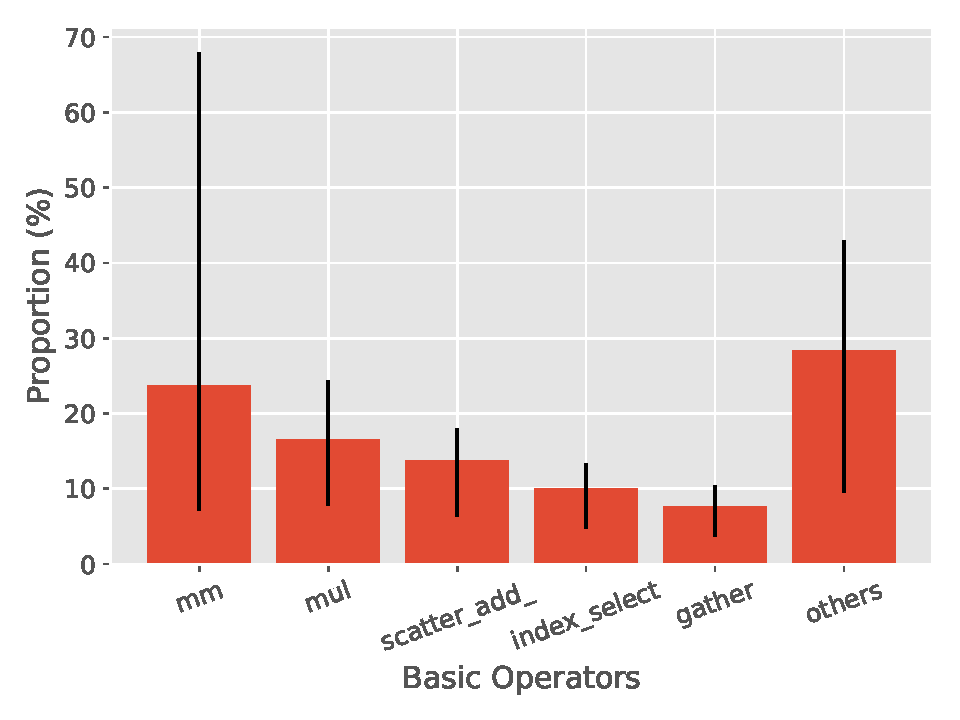
\includegraphics[height=4cm]{figs/experiments/exp_top_basic_ops_gcn.pdf}}
    \subfloat[GGNN]{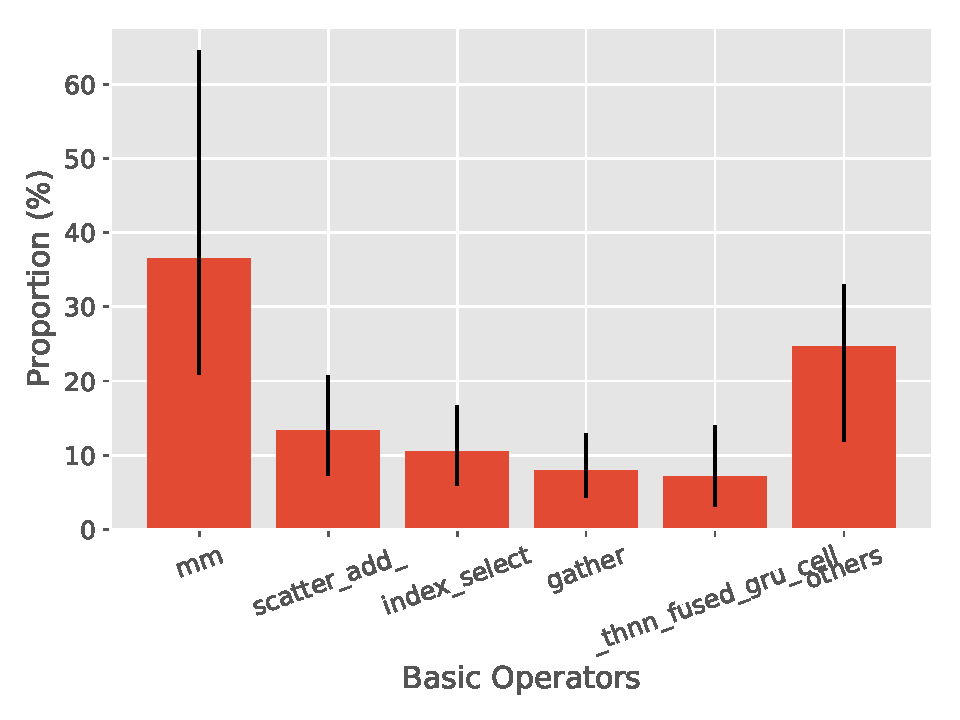
\includegraphics[height=4cm]{figs/experiments/exp_top_basic_ops_ggnn.pdf}}\\
    \subfloat[GAT]{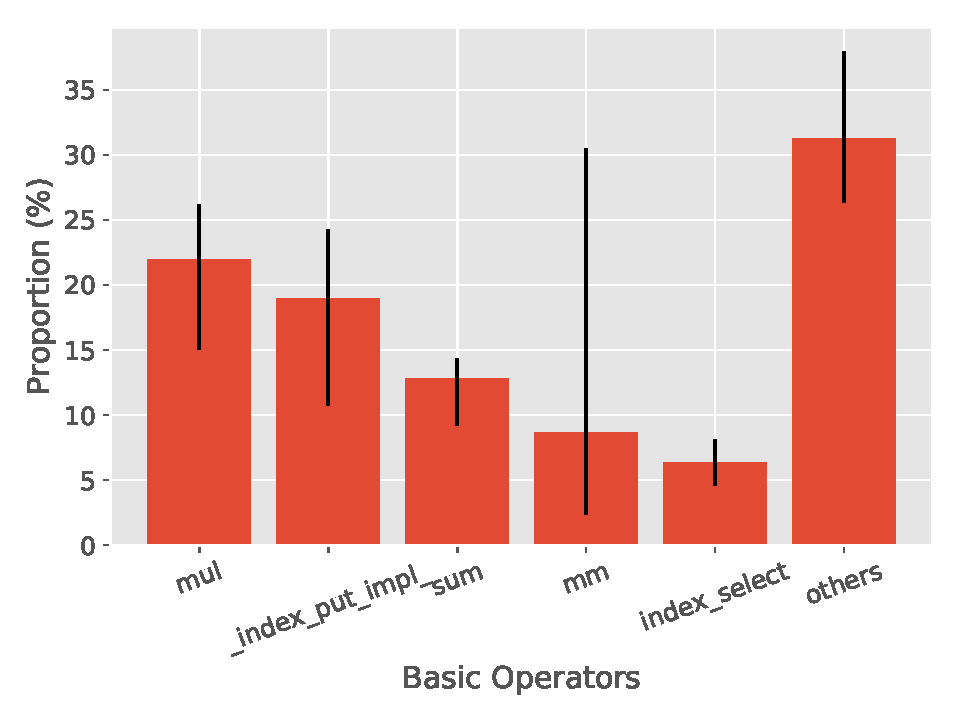
\includegraphics[height=4cm]{figs/experiments/exp_top_basic_ops_gat.pdf}}
    \subfloat[GaAN]{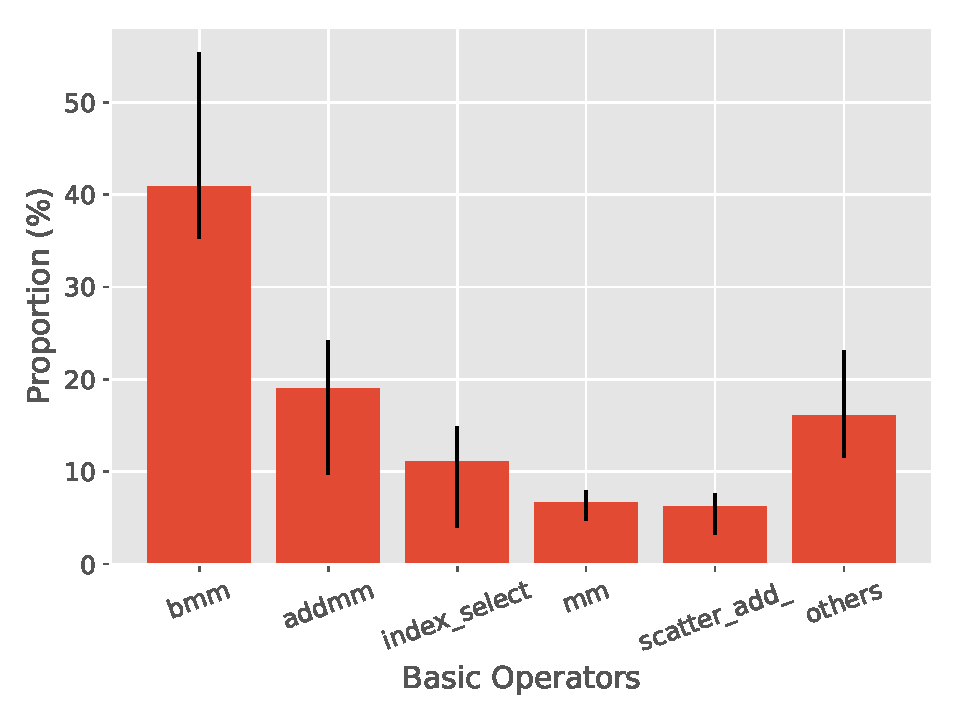
\includegraphics[height=4cm]{figs/experiments/exp_top_basic_ops_gaan.pdf}}
    \caption{Top 5 time-consuming basic operators of typical GNNs. The time proportion of each basic operator is averaged over all graphs with the error bar indicating the maximal and the minimal.}
    \label{fig:exp_top_basic_ops}
\end{figure}

\paragraph{GCN}
The most time-consuming basic operator is the matrix multiplication \texttt{mm} used in the vertex updating function $\gamma$.
The elementwise multiplication \texttt{mul} used in the messaging function $\phi$ is also time-consuming.
The other three operators are used in the edge calculation stage: \texttt{scatter\_add\_} for the aggregation step in the forward phase, \texttt{gather} for the aggregation step in the backward phase, and \texttt{index\_select} for the collection step.
For GCN, the basic operators related to the edge calculation stage consume the majority of the training time.

\paragraph{GGNN}
The top basic operator is \texttt{mm} used in the vertex updating function $\gamma$.
Due to its high time complexity, the proportion of the \texttt{mm} is much higher than the other operators.
The \texttt{thnn\_fused\_gru\_cell} operator used in the backward phase of $\gamma$ is also noticeable.
The other three operators are used in the edge calculation stage.

\paragraph{GAT}
All the top basic operators except for \texttt{mm} are related to the edge calculation stage.
The \texttt{mm} operator is used in the vertex updating function $\gamma$.

\paragraph{GaAN}
The top basic operator is \texttt{bmm} used in the messaging function $\phi$.
The \texttt{addmm} operator and the \texttt{mm} operator are used in both the vertex and the edge calculation stages, where the edge calculation stage is dominant.

In general, the most time-consuming operator in the four GNNs, is still the matrix multiplication \texttt{mm} and the elementwise multiplication \texttt{mul}, \emph{making GNN training suitable for GPUs}.
Although the aggregation step in the edge calculation stage is relatively simple (like sum and mean), the related operators \texttt{scatter\_add} and \texttt{gather} still consume a certain amount of the time.
The operators have to synchronize between hardware threads to avoid updating the same aggregated vector at the same time. They also conduct non-regular memory access with the access pattern determined by the edge set dynamically.
For GPUs, they are less efficient than \texttt{mm}.
The index-based selection \texttt{index\_select} operator from the collection step consume around 10\% of the time in all GNNs.
Though GPUs have high on-chip memory bandwidth, improving the efficiency of \texttt{scatter\_add}/\texttt{gather}/\texttt{index\_select} can benefit the training of all kinds of GNNs.

\paragraph{Summary}
The GNN training is suitable for GPUs.
\textbf{The edge calculation stage is the main performance bottleneck in most cases}, except for training GNNs with high vertex calculation complexity on low-average-degree graphs.
The performance bottleneck in the edge calculation stage depends on the time complexity of the messaging function $\phi$.
\begin{itemize}
    \item If the time complexity of $\phi$ is \textbf{high}, the \textbf{efficiency of $\phi$} limits the performance. Reducing its computation cost (via optimizing its implementation or modifying the algorithm) can significantly reduce the training time.
    \item If the time complexity of $\phi$ is \textbf{low}, the \textbf{collection step} and the \textbf{aggregation step} limit the performance. The collection step involves lots of data movement. The aggregation step suffers from data synchronization and non-regular data access. Optimizing their implementations can significantly reduce the training time.
\end{itemize}

\subsection{Memory Usage Analysis}
\label{sec:memory_usage_analysis}

During the GNN training, all data (including datasets and intermediate results) are stored in the on-chip memory of the GPU.
Compared with the main memory on the host side, the capacity of the GPU memory is very limited.
\emph{The GPU memory capacity limits the scales of the graphs that a GPU can train GNNs on}.
For example, GaAN is unable to train on \texttt{cph} dataset due to the out of memory exception.

\begin{figure}[tbp]
    \centering
    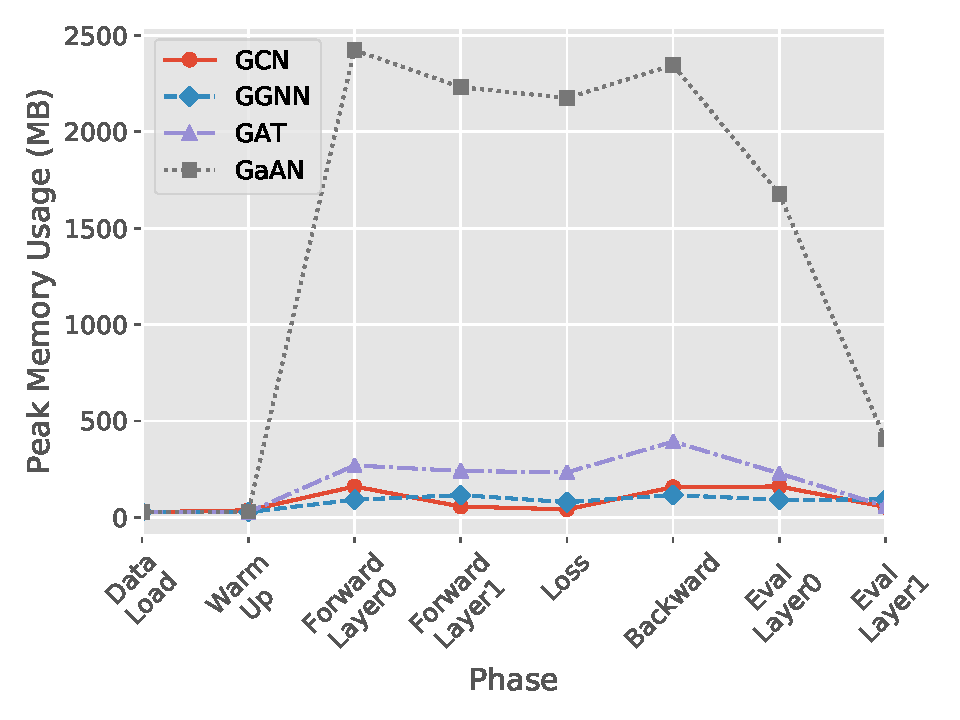
\includegraphics[height=5cm]{figs/experiments/exp_memory_usage_stage_amp.pdf}
    \caption{Memory usage of each phase. Dataset: \texttt{amp}.}
    \label{fig:exp_memory_usage_stage_amp}
\end{figure}

\begin{figure}[tbp]
    \centering
    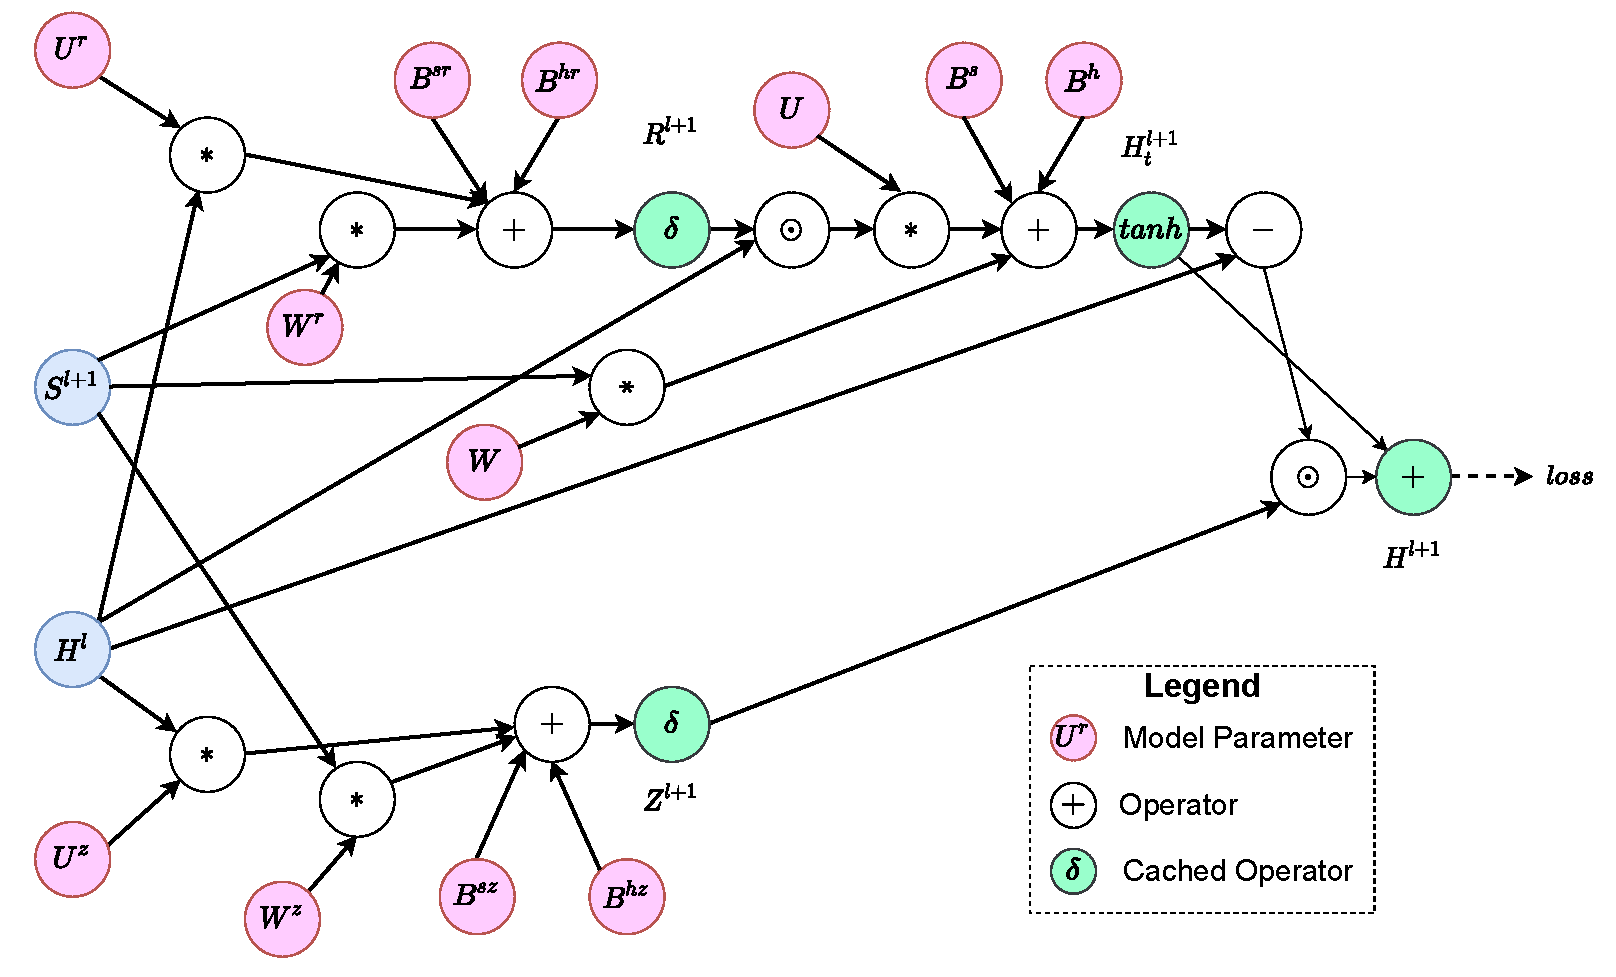
\includegraphics[height=4.5cm]{figs/illustration/ggnn_vertex_func_computation_graph.pdf}
    \caption{Computation graph of the vertex updating function $\gamma$ of GGNN.}
    \label{fig:ggnn_vertex_func_computation_graph}
\end{figure}

\figurename~\ref{fig:exp_memory_usage_stage_amp} shows the peak memory usage of each phase in the GNN training on the \texttt{amp} dataset.
The trend is similar on the other datasets.
\emph{The GNN training achieves its peak memory usage in the forward and the backward phases}.
The forward phase generates lots of intermediate results.
Some key intermediate results are cached, increasing memory usage.
The cached results are used in the gradient calculation in the backward phase.
\figurename~\ref{fig:ggnn_vertex_func_computation_graph} shows the computation graph of the vertex updating function $\gamma$ of GGNN.
The computation graph has a large number of operators. Each operator generates an intermediate tensor.
Some key intermediate tensors are cached.
The cached tensors are the main source of memory usage in the loss phase.
By the end of the backward phase, the cached tensors are released.
Since the evaluation phase does not need to calculate the gradients, it does not cache intermediate tensors.
Its memory usage declines sharply.

\begin{figure}[tbp]
    \centering
    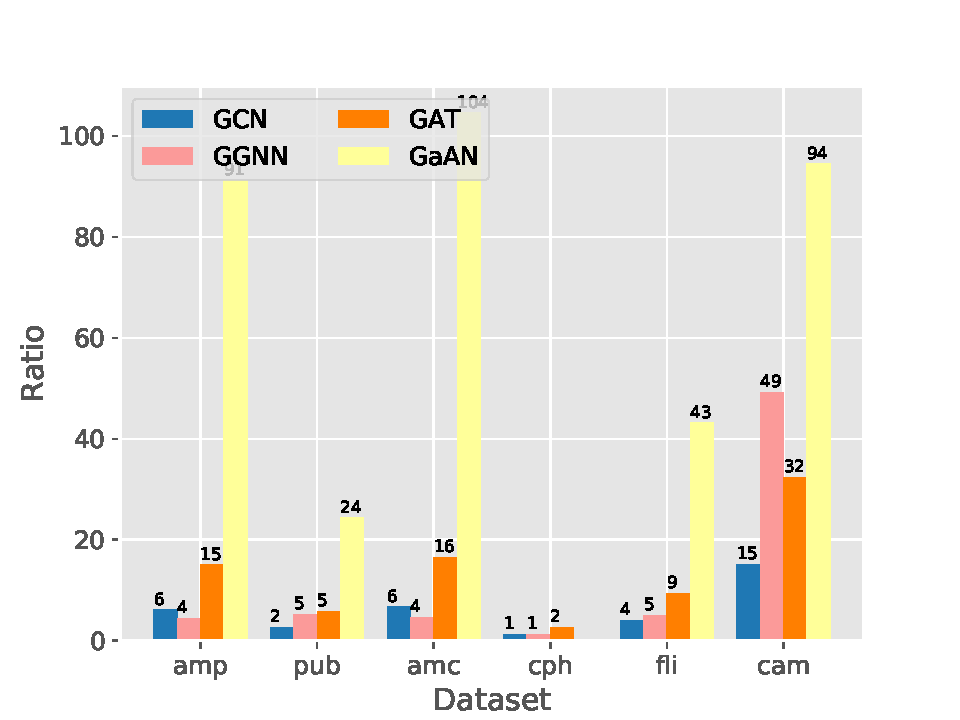
\includegraphics[height=5cm]{figs/experiments/exp_memory_expansion_ratio.pdf}
    \caption{Memory expansion ratios of typical GNNs.}
    \label{fig:exp_memory_expansion_ratio}
\end{figure}

The peak memory usage during the GNN training far exceeds the size of the dataset itself.
We define the \emph{memory expansion ratio} (MER) as the ratio of the peak memory usage during the training to the memory usage after loading the dataset.
\figurename~\ref{fig:exp_memory_expansion_ratio} compares MER of different GNNs.
GCN has the lowest MER (up to 15) while GaAN has the highest MER (up to 104).
\emph{The high MER limits the data scalability of GNNs}, making GPUs unable to handle big graphs.

\begin{figure}[tbp]
    \centering
    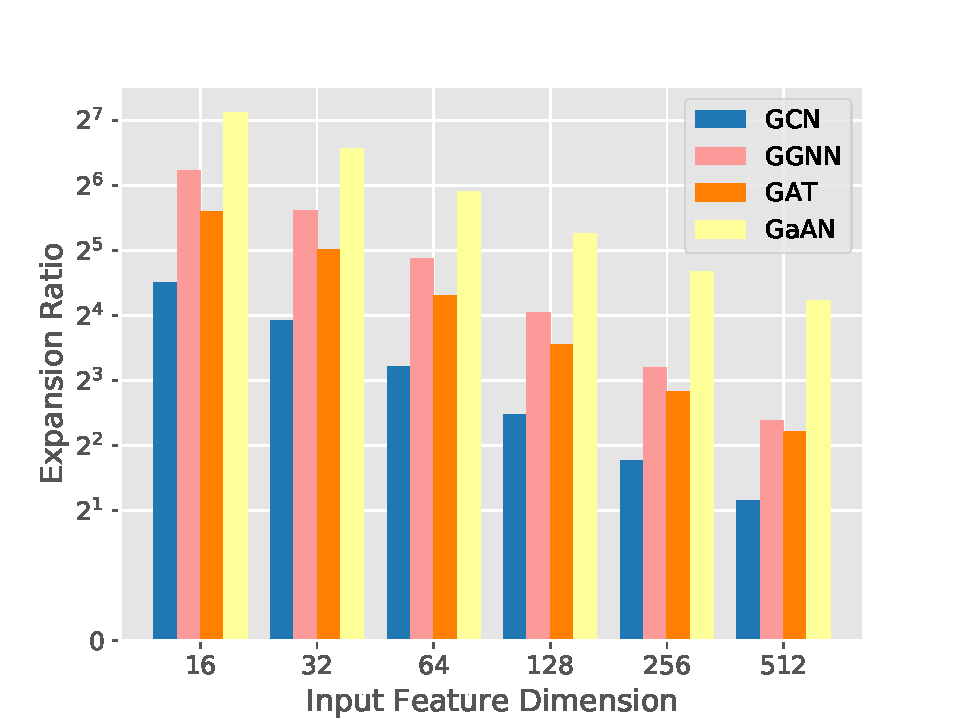
\includegraphics[height=5cm]{figs/experiments/exp_memory_expansion_ratio_input_feature_dimension_com-amazon.pdf}
    \caption{Memory expansion ratio under different dimensions of the input feature vectors. Dataset: \texttt{cam}.}
    \label{fig:exp_memory_expension_ratio_input_feature_dimension}
\end{figure}

\figurename~\ref{fig:exp_memory_expansion_ratio} also indicates that the same GNN has different MERs for different datasets.
Two characteristics of a dataset affect the MER: the dimension of the input feature vector and the average degree.

Given the same graph, the scales of the intermediate results are mainly affected by the hyper-parameters of the GNN.
If the dimension of the input feature vectors is high (like the \texttt{cph} dataset), the size of the dataset is large.
The size may become comparable to the scales of the intermediate results,  making the MER low.
To find out how the dimension affects the MER, we generated random input feature vectors with different dimensions for the \texttt{cam} dataset and measured the MER in \figurename~\ref{fig:exp_memory_expension_ratio_input_feature_dimension}.
For a GNN under the same hyper-parameters, \emph{the MER decreases as the dimension of the input feature vectors increases}.

\begin{figure}[tbp]
    \centering
    \subfloat[Peak memory usage]{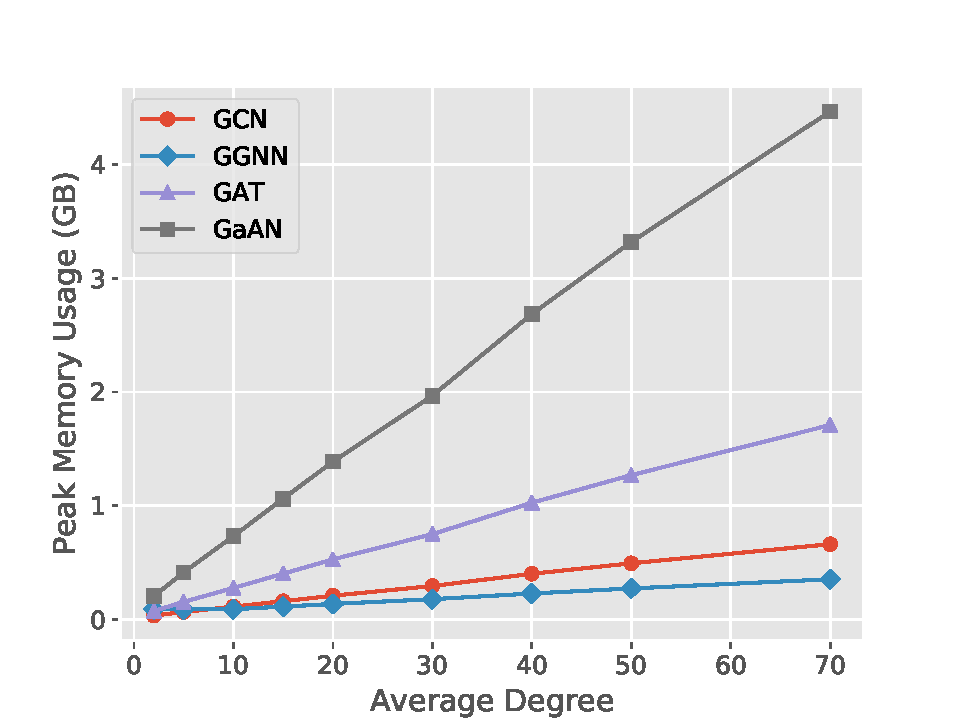
\includegraphics[height=4cm]{figs/experiments/exp_memory_expansion_ratio_input_graph_number_of_edges_peak_memory.pdf}}
    \subfloat[Memory expansion ratio]{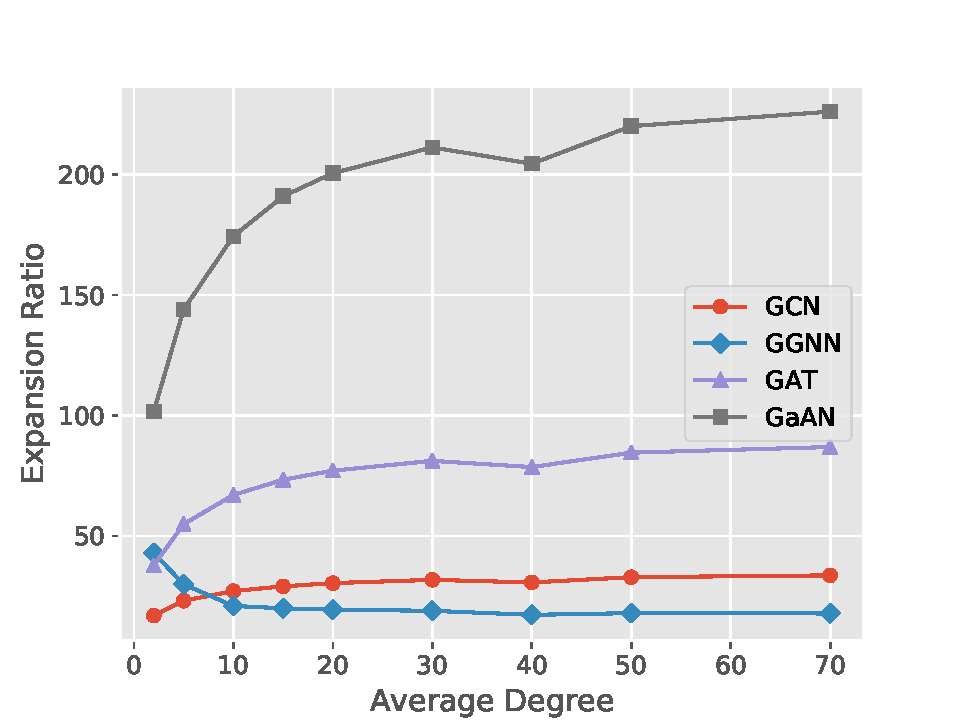
\includegraphics[height=4cm]{figs/experiments/exp_memory_expansion_ratio_input_graph_number_of_edges_expansion_ratio.pdf}}
    \caption{Memory usage under different average degrees of the graph. The graph was generated with the R-MAT generator fixing the number of vertices at 10K and the dimension of the input feature vectors at 32.}
    \label{fig:exp_memory_expansion_ratio_input_graph_number_of_edges}
\end{figure}

The average degree of the graph also affects MER by influencing the relative scales of the intermediate results from the edge/vertex calculation stages.
Fixing the number of vertices $|\mathcal{V}|$, we used the R-MAT generator to generate random graphs with different average degrees.
\figurename~\ref{fig:exp_memory_expansion_ratio_input_graph_number_of_edges} shows how the memory usage changes according to the average degrees.
As the average degree $\bar{d}$ increases, the number of edges $|\mathcal{E}|$ increases and the peak memory usage increases \emph{linearly} with $\bar{d}$.
The edge calculation stage gradually dominates the memory usage and \emph{the MER converges to a stable value}.
The stable value is determined by the complexity of the edge calculation stage.
Except for GGNN, the MER of the other GNNs increases as $\bar{d}$ increases.
As GGNN has high vertex calculation complexity, the MER related to the vertex calculation stage is much larger than the edge calculation stage.
When the edge calculation stage dominates the memory usage, its MER becomes smaller.

\begin{figure}[tbp]
    \centering
    \subfloat[Peak memory usage]{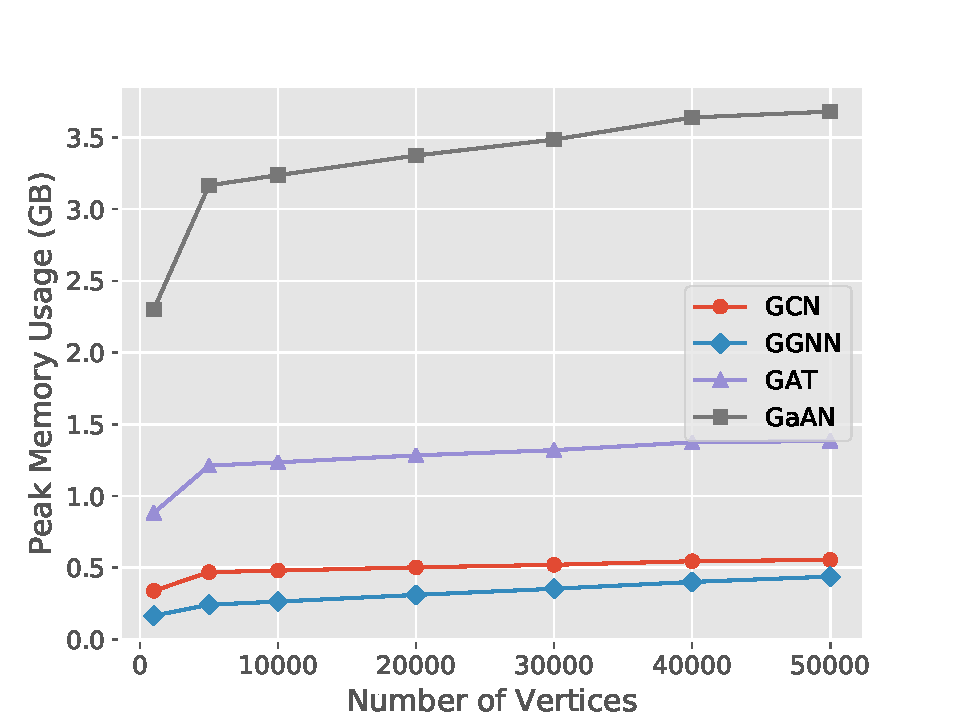
\includegraphics[height=4cm]{figs/experiments/exp_memory_expansion_ratio_input_graph_number_of_vertices_fixed_edge_peak_memory.pdf}}
    \subfloat[Memory expansion ratio]{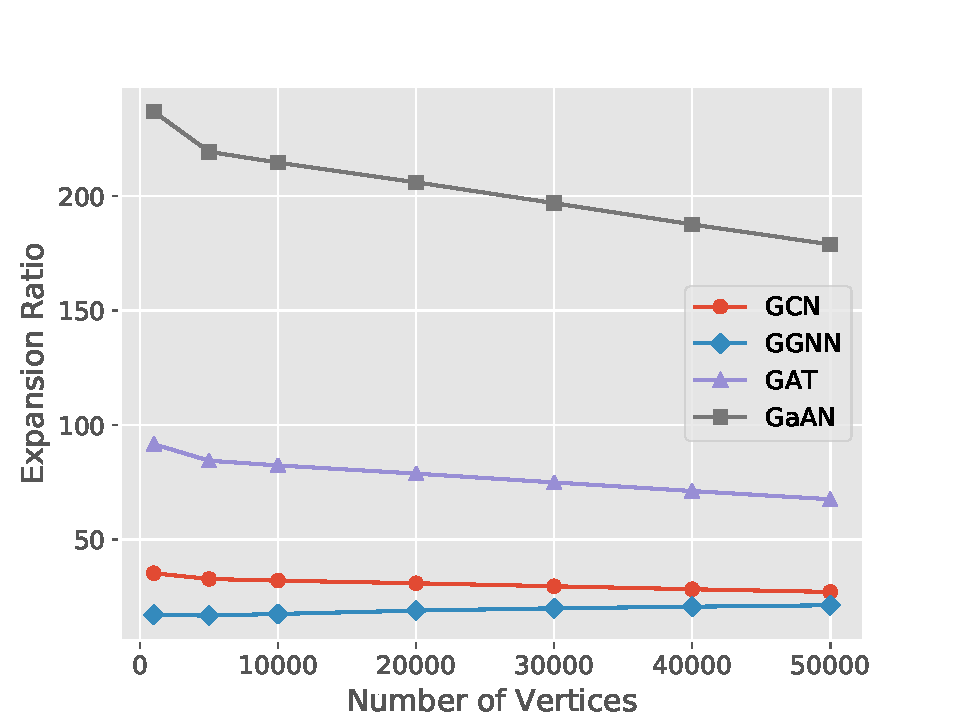
\includegraphics[height=4cm]{figs/experiments/exp_memory_expansion_ratio_input_graph_number_of_vertices_fixed_edge_expansion_ratio.pdf}}
    \caption{Memory usage under different numbers of vertices of the graph. The graph was generated with the R-MAT generator fixing the number of edges at 500K and the dimension of the input feature vectors at 32.}
    \label{fig:exp_memory_expansion_ratio_input_graph_number_of_vertices_fixed_edge}
\end{figure}

We also fixed the number of edges $|\mathcal{E}|$ in the graphs and generated random graphs with different $|\mathcal{V}|$.
\figurename~\ref{fig:exp_memory_expansion_ratio_input_graph_number_of_vertices_fixed_edge} shows how the memory usage changes according to $|\mathcal{V}|$.
All GNNs are insensitive to the changes in $|\mathcal{V}|$ compared to $|\mathcal{E}|$.
Except for GGNN, the MERs of the other GNNs decline as $|\mathcal{V}|$ increases because the scales of the datasets increase more quickly than the scales of the intermediate results.
As GGNN has high vertex calculation complexity, the scales of the intermediate results are much more sensitive to $|\mathcal{V}|$.
It indicates that \emph{the intermediate results of the edge calculation stage dominated the memory usage during the GNN training}.

\paragraph{Summary}
The \emph{high} memory expansion ratio severely restrictes the data scalability of the GNN training.
The memory usage mainly comes from the intermediate results of the \emph{edge calculation stage}.
Fixing the number of vertices, the memory usage increases \emph{linearly} along with the number of edges.
Optimizing the memory usage of the edge calculation stage can significantly reduce the memory expansion ratio.
Fixing the GNN structures and the hyper-parameters, increasing the dimension of the input feature vectors can also reduce the memory expansion ratio.

\subsection{Effects of Sampling Techniques on Performance}
\label{sec:effects_of_sampling_techniques_on_performance}

With the sampling techniques, GNNs can be trained in a mini-batch manner.
Each mini-batch updates the model parameters based on a small subgraph sampled from the original input graph.
Thus, the training time per batch and the peak memory usage during the training should both decline significantly.

In the implementation in PyG, the GNN model and the dataset resides on the GPU side.
To process each epoch, PyG samples the original dataset in the main memory and generates several batches.
Each batch is a small subgraph of the dataset.
To train on each batch, PyG sends the sampled subgraph to the GPU, calculates the gradients on the subgraph, and updates the model parameters directly on GPU.
With the sampling techniques, the model parameters are updated by a stochastic gradient descent optimizer.
PyG conducts the evaluation phase every several epochs (either on the CPU side or the GPU side) to determine whether to stop the training.
In this section, the experiments focus on the training phase of each batch.

\begin{figure}[tbp]
    \centering
    \subfloat[Neighbor sampler]{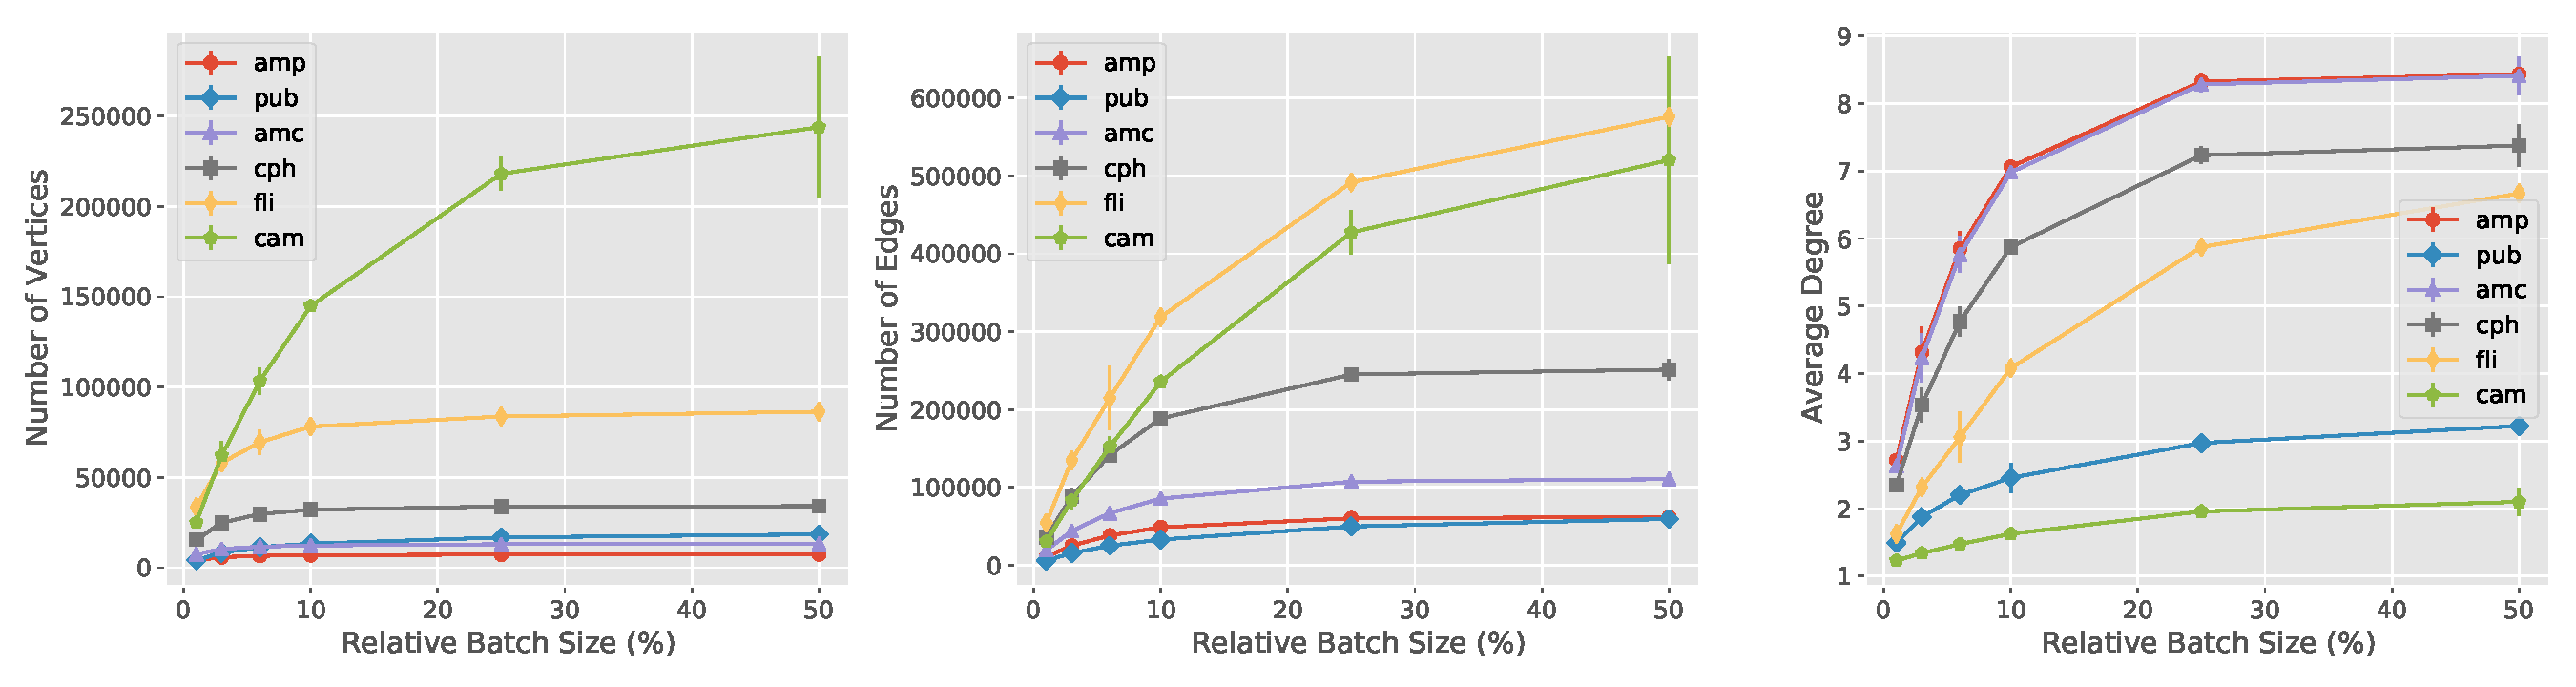
\includegraphics[height=4cm]{figs/experiments/exp_sampling_minibatch_realtive_graph_info_graphsage_gcn.pdf}} \\
    \subfloat[Cluster sampler]{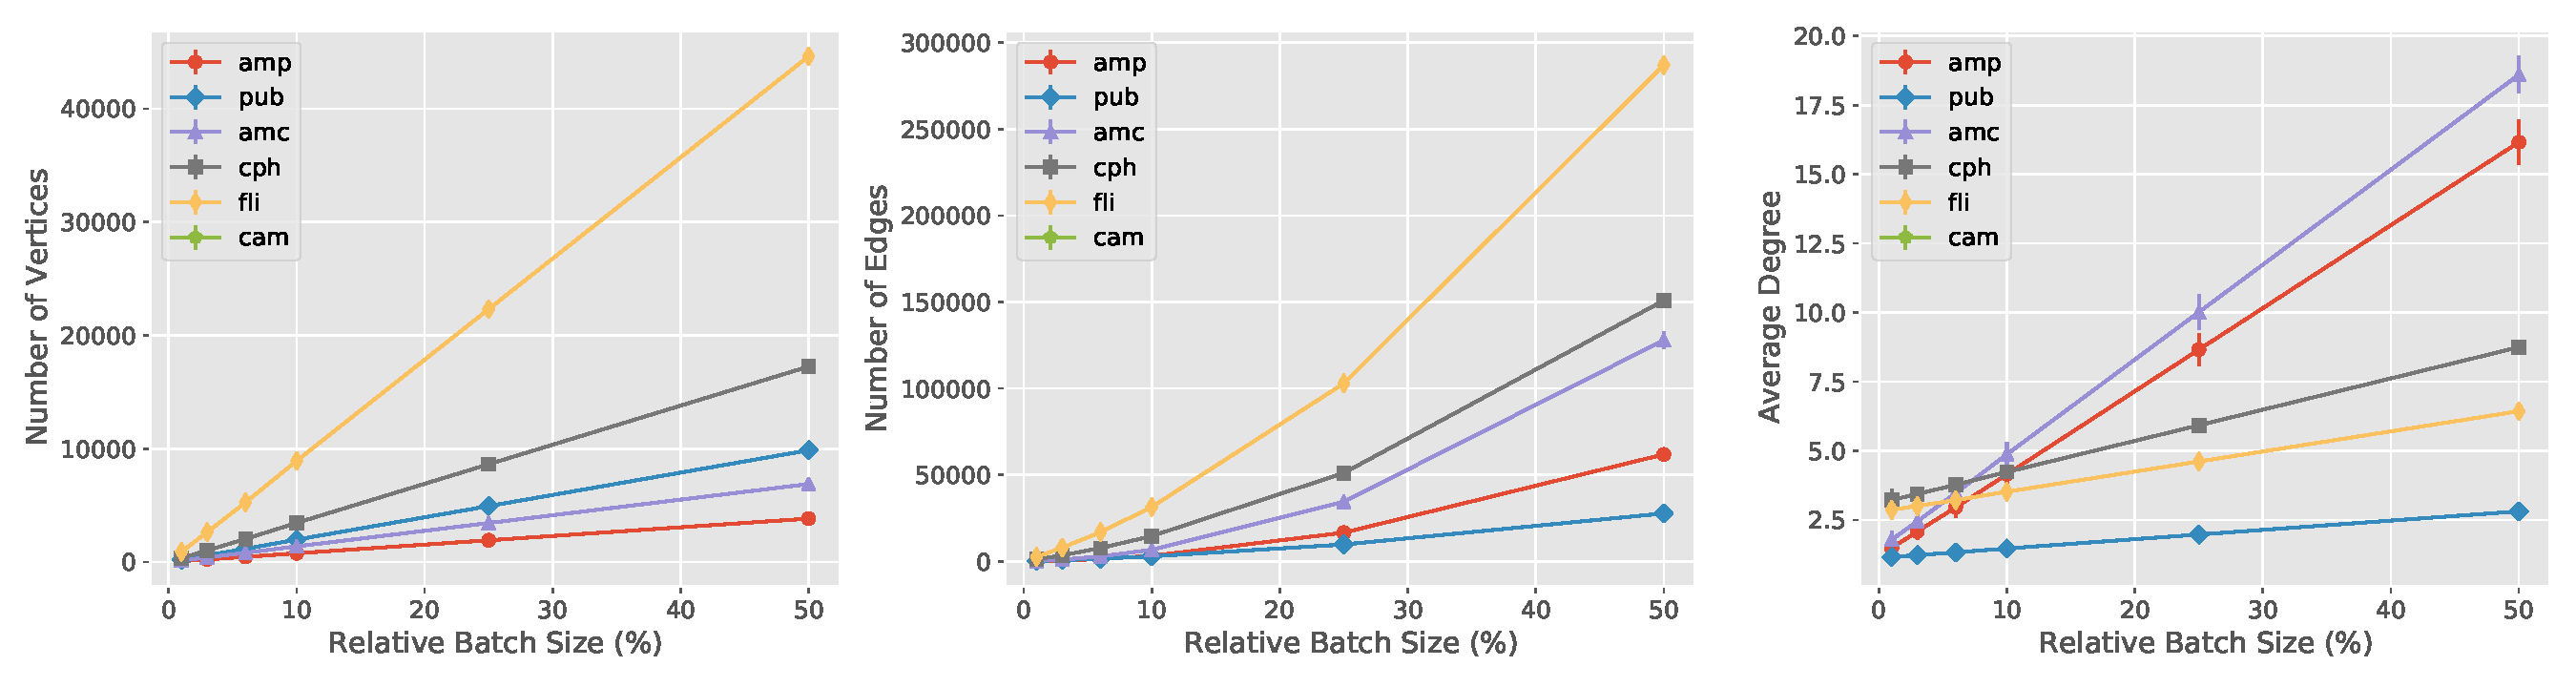
\includegraphics[height=4cm]{figs/experiments/exp_sampling_minibatch_realtive_graph_info_cluster_gcn.pdf}}
    \caption{Sizes of the sampled subgraphs under different batch sizes. Each batch size was sampled 50 times and the average value was reported. The error bar indicates the standard deviation. The batch size is relative to the full graph.}
    \label{fig:exp_sampling_minibatch_graph_info}
\end{figure}

\figurename~\ref{fig:exp_sampling_minibatch_graph_info} shows how the size of the sampled subgraph changes with the batch size.
For the neighbor sampler, the relative batch size is the proportion of the sampled vertices of the last GNN layer in $|\mathcal{V}|$.
For the cluster sampler, the relative batch size is the proportion of the sampled partitions to all partitions of the graph.
The neighbor sampler is very sensitive to the batch size.
As the batch size increases, the size of the sampled subgraph first increases quickly and then stabilizes.
The cluster sampler is much less sensitive compared to the neighbor sampler.
The number of vertices and the average degree of the sampled subgraphs increases linearly with the batch size.

\begin{figure}[tbp]
    \centering
    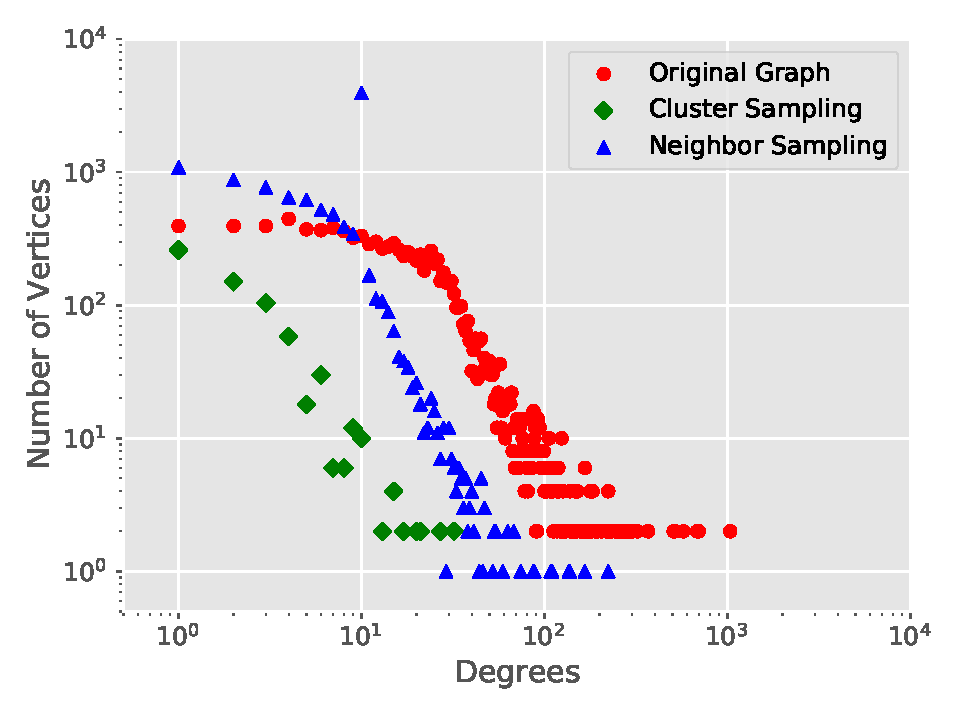
\includegraphics[width=0.4\columnwidth]{figs/experiments/exp_sampling_minibatch_degrees_distribution_amazon-photo.pdf}
    \caption{Vertex degree distribution of the sampled subgraph (relative batch size: 6\%) and the original graph. Dataset:\texttt{amp}.}
    \label{fig:exp_sampling_minibatch_degrees_distribution}
\end{figure}

It is worth noting that the average degree of the sampled subgraph is \emph{much lower} than the average degree of the whole graph, especially when the relative batch size is low.
Taking the neighbor sampler with the relative batch size of 6\% as an example, the average degree of the \texttt{amp} dataset is 31.1, but the average degree of the sampled subgraph is only 5.8.
For the cluster sampler, the average degree is 3.0.
\figurename~\ref{fig:exp_sampling_minibatch_degrees_distribution} compares the degree distribution of the sampled subgraphs with the original graph.
The slopes of the curves are similar.
It indicates that the sampled subgraphs still follow the power-law degree distribution.
However, there are much less vertices in the sampled subgraphs, significantly lowering the average degrees.
According to the experimental results in Section~\ref{sec:training_time_breakdown}, if the average degree becomes lower, the proportion of the training time spent on the vertex calculation stage will become higher, especially for GGNN.

\begin{figure}[tbp]
    \centering
    \subfloat[Neighbor sampler on \texttt{amc}]{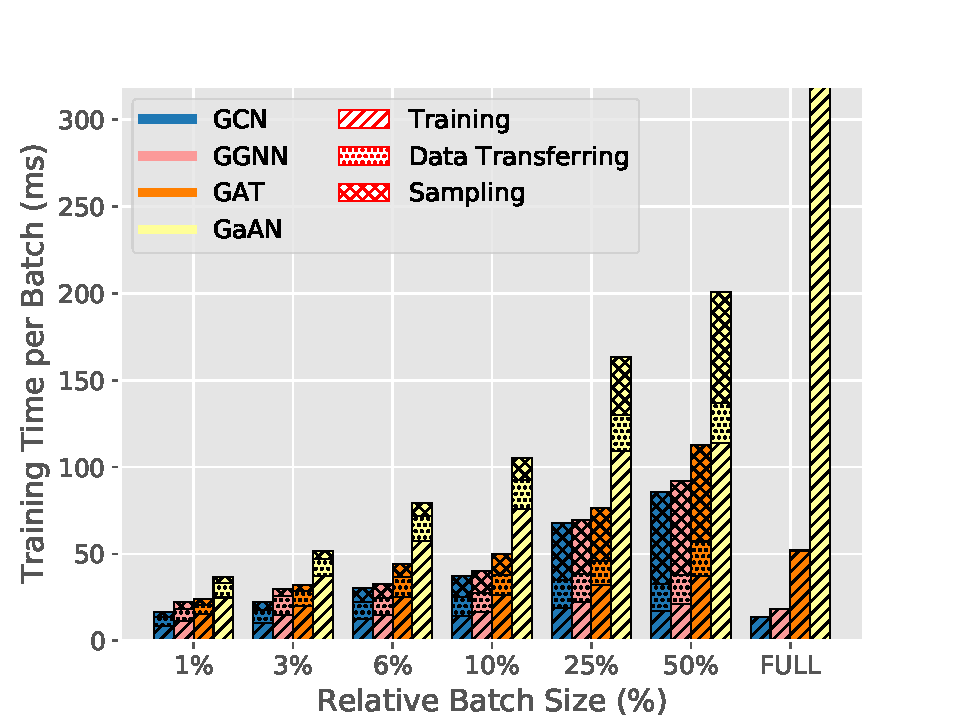
\includegraphics[height=5cm]{figs/experiments/exp_sampling_relative_batch_size_train_time_stack_graphsage_amazon-computers.pdf}}
    \subfloat[Neighbor sampler on \texttt{fli}]{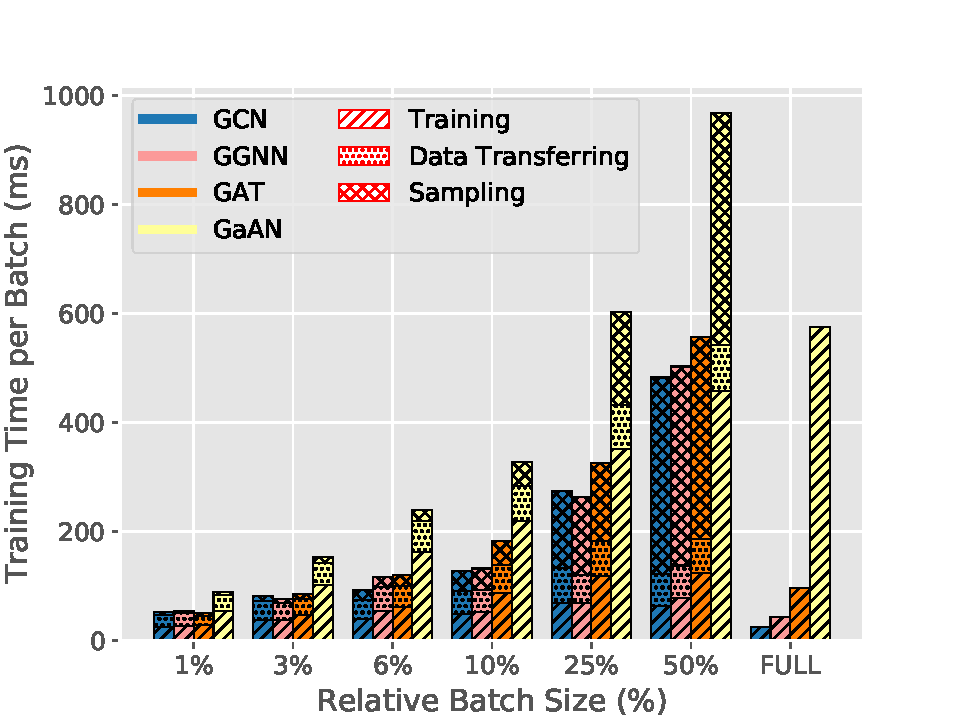
\includegraphics[height=5cm]{figs/experiments/exp_sampling_relative_batch_size_train_time_stack_graphsage_flickr.pdf}} \\
    \subfloat[Cluster sampler on \texttt{amc}]{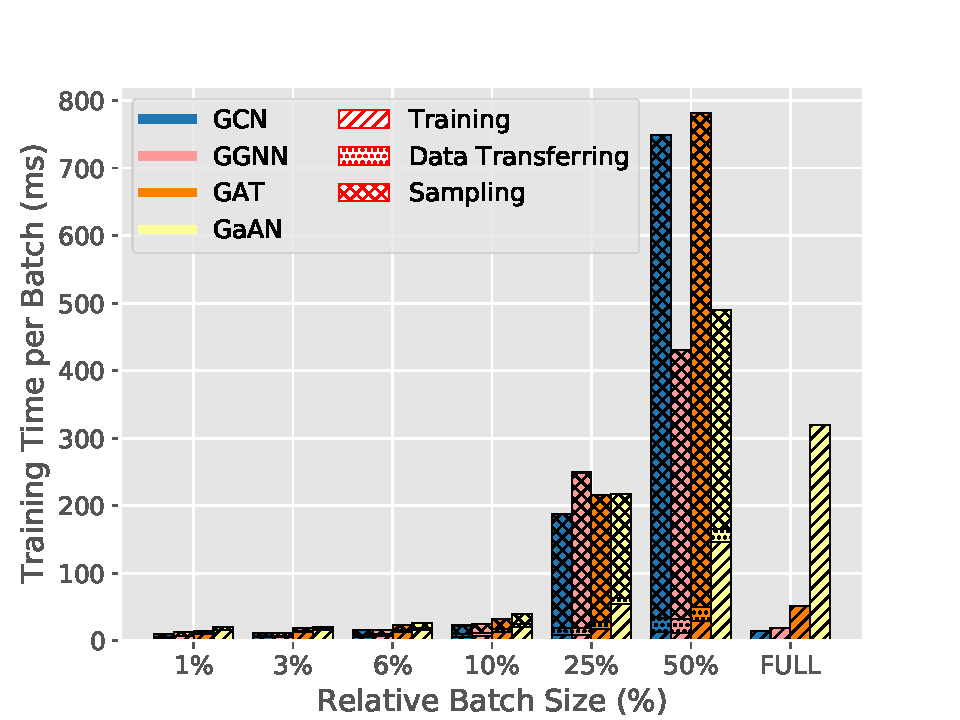
\includegraphics[height=5cm]{figs/experiments/exp_sampling_relative_batch_size_train_time_stack_cluster_amazon-computers.pdf}}
    \subfloat[Cluster sampler on \texttt{fli}]{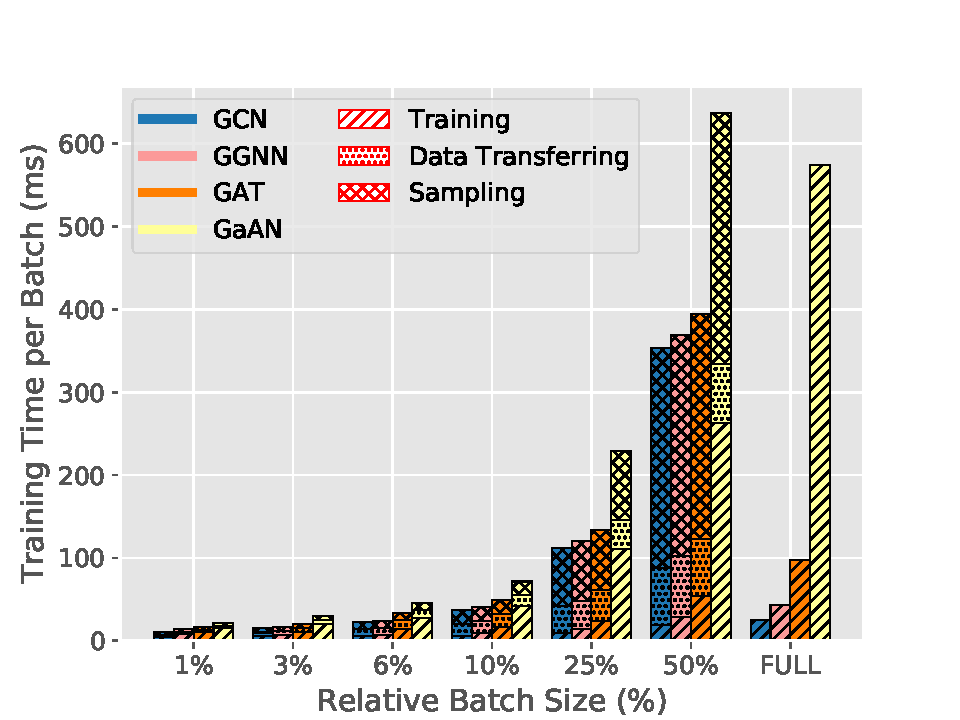
\includegraphics[height=5cm]{figs/experiments/exp_sampling_relative_batch_size_train_time_stack_cluster_flickr.pdf}}
    \caption{Training time per batch breakdown. FULL means that the full graph participates in the training.}
    \label{fig:exp_sampling_batch_train_time}
\end{figure}

To find out the performance bottleneck with the sampling techniques, we decompose the training time per batch into three phases: \emph{sampling} on the CPU, \emph{transferring} sampled subgraphs from the CPU to the GPU and \emph{training} with the subgraphs on GPU.
\figurename~\ref{fig:exp_sampling_batch_train_time} shows the time breakdown of the four GNNs under different relative batch sizes.
For the neighbor sampler, the sampling technique reduces the training time per batch only when the batch size is very small.
When the batch becomes bigger, the sampling and the data transferring phases introduce noticeable overheads, making the training time exceed the full-batch training.
For the clustering sampler, the sampled subgraph is smaller than the neighbor sampler under the same relative batch size.
The reduction in the training time is more obvious than the neighbor sampler.
However, the overheads increase quickly as the relative batch size increase.
The training time under the 25\% relative batch size already exceede the time of full-batch training.
The experimental results indicate that the current implementation of the sampling techniques in PyG is inefficient.
When the batch size is slightly big, more than 50\% of the time has been spent on sampling and data transferring.
\emph{The sampling techniques are only efficient under small batch sizes.}

\begin{figure}[tbp]
    \centering
    \subfloat[Neighbor sampler on \texttt{amc}]{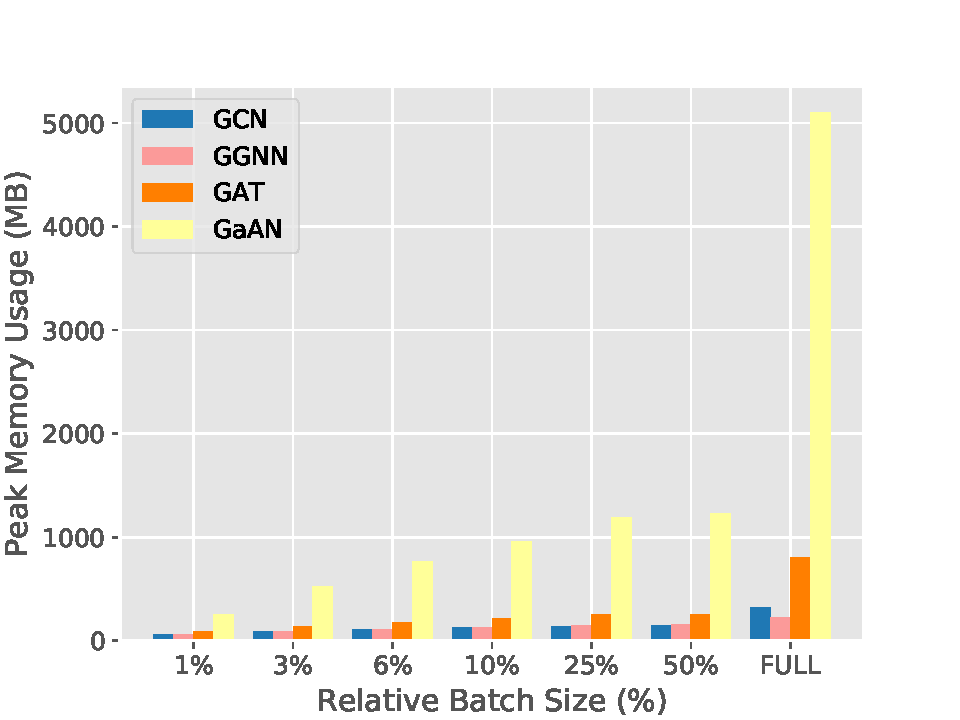
\includegraphics[height=4cm]{figs/experiments/exp_sampling_memory_usage_relative_batch_size_graphsage_amazon-computers_peak_memory.pdf}}
    \subfloat[Neighbor sampler on \texttt{fli}]{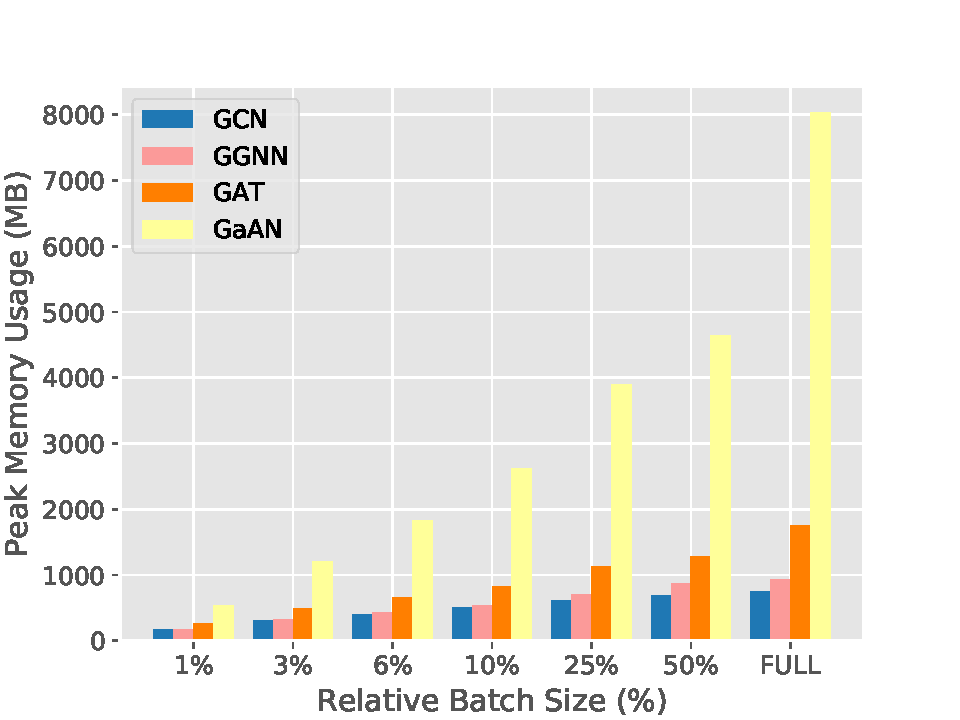
\includegraphics[height=4cm]{figs/experiments/exp_sampling_memory_usage_relative_batch_size_graphsage_flickr_peak_memory.pdf}} \\
    \subfloat[Cluster sampler on \texttt{amc}]{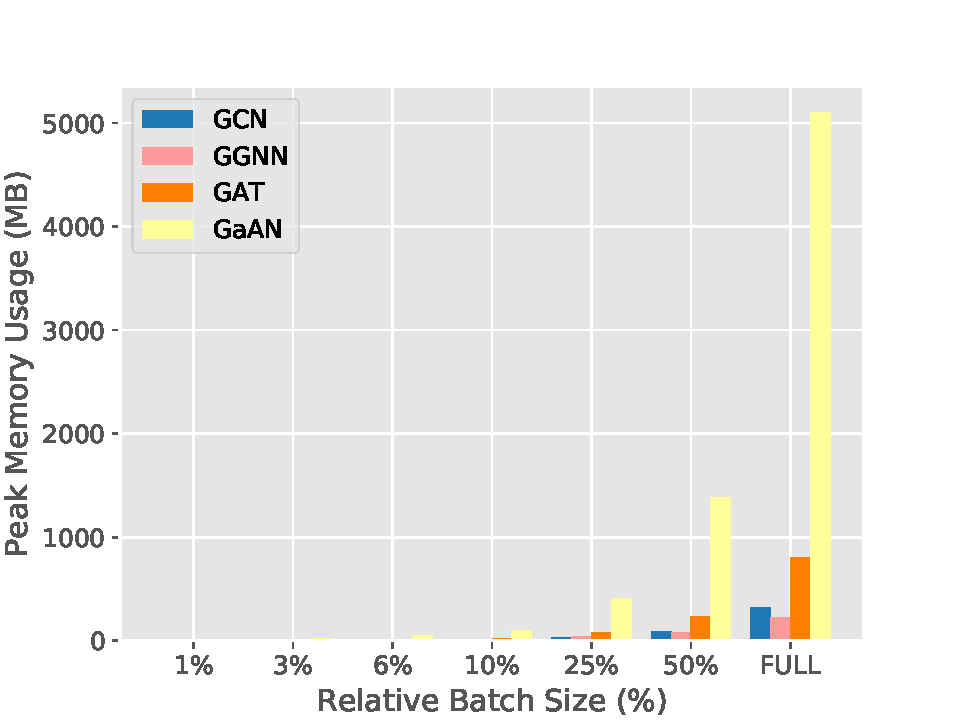
\includegraphics[height=4cm]{figs/experiments/exp_sampling_memory_usage_relative_batch_size_cluster_amazon-computers_peak_memory.pdf}}
    \subfloat[Cluster sampler on \texttt{fli}]{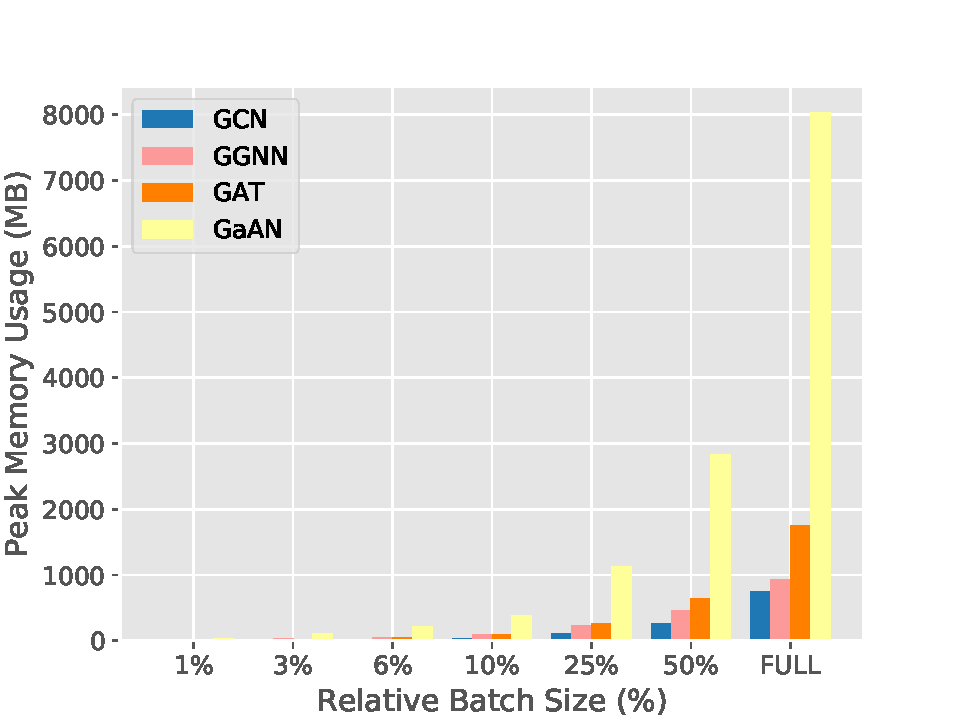
\includegraphics[height=4cm]{figs/experiments/exp_sampling_memory_usage_relative_batch_size_cluster_flickr_peak_memory.pdf}}
    \caption{Peak memory usage under different batch sizes. FULL means the full graph participates in the training.}
    \label{fig:exp_sampling_memory_usage}
\end{figure}

The main advantage of the sampling technique is \emph{reducing the peak memory usage} during the training.
\figurename~\ref{fig:exp_sampling_memory_usage} shows the memory usage under different batch sizes.
The peak memory usage declines significantly even under big batch sizes.
The sampling techniques make training GNNs on big graphs possible for GPUs.

\begin{figure}[tbp]
    \centering
    \includegraphics[height=5cm]{figs/experiments/exp_small_graph_train_time.pdf}
    \caption{Training time per epoch on small random graphs. For each number of vertices, we generated 50 random R-MAT graphs with the average degree of 4.0 and reported the average training time per epoch (without the evaluation phase). The error bar indicates the standard deviation.}
    \label{fig:exp_small_graph_train_time}
\end{figure}

The disadvantage of the sampling technique is wasting GPU resources.
As the sampling techniques are only effective under small batch sizes, the sampled subgraphs will be very small in those cases.
They cannot make full use of the computing power of a GPU.
To simulate the situation, we generated random graphs with few vertices and measured the training time per epoch in \figurename~\ref{fig:exp_small_graph_train_time}.
As the number of vertices increases, the training time is almost unchanged except for GaAN.
The training time of GaAN increases only with $|\mathcal{V}| \geq 4000$.


\paragraph{Summary}
The sampled subgraphs have lower average degrees than the whole graph.
With small batch sizes, the sampling techniques can significantly reduce the training time per batch and the peak memory usage during the training.
However, small batch sizes cannot make full use of the computing power of a GPU.
With big batch sizes, the current implementation of the sampling techniques in PyG is inefficient.
The time spent on the sampling phase and the data transferring phase even exceeds the training phase.
